%%%%%%%%%%%%%%%%%%%%%%%%%%%%%%%%%%%%%%%%

%----------------------------------------------------------------------------------------
%	PACKAGES AND OTHER DOCUMENT CONFIGURATIONS
%----------------------------------------------------------------------


% Line spacing, alternatives: onehalfspacing or doublespacing, singlespacing
% The default document font size, options: 10pt, 11pt, 12pt
%oneside, % Two side (alternating margins) for binding by default, uncomment to switch to one side
%liststotoc, % Uncomment to add the list of figures/tables/etc to the table of contents
%toctotoc, % Uncomment to add the main table of contents to the table of contents
%parskip, % Uncomment to add space between paragraphs
%nohyperref, % Uncomment to not load the hyperref package
% Uncomment to get a line under the header
%chapterinoneline, % Uncomment to place the chapter title next to the number on one line
%consistentlayout, % Uncomment to change the layout of the declaration, abstract and acknowledgements pages to match the default layout

\documentclass[11pt, twoside, english, doublespacing, nolistspacing, headsepline]{MastersDoctoralThesis} 

\usepackage[utf8]{inputenc} % Required for inputting international characters
\usepackage[T1]{fontenc} % Output font encoding for international characters

%\usepackage{mathpazo} % Use the Palatino font by default

\usepackage[style=numeric,sorting=none]{biblatex}
\addbibresource{example.bib} % The filename of the bibliography

%\usepackage[autostyle=true]{csquotes} % Required to generate language-dependent quotes in the bibliography

\parindent 0mm
%----------------------------------------------------------------------------------------
%	MARGIN SETTINGS
%----------------------------------------------------------------------------------------

\geometry{
	paper=a4paper, % Change to letterpaper for US letter
	inner=4.0cm, % Inner margin
	outer=2.5cm, % Outer margin
	bindingoffset=.5cm, % Binding offset
	top=1.5cm, % Top margin
	bottom=1.5cm, % Bottom margin
	%showframe, % Uncomment to show how the type block is set on the page
}

%----------------------------------------------------------------------------------------
%	THESIS INFORMATION
%----------------------------------------------------------------------------------------

\thesistitle{Measurement of vertical betatron oscillations using the straw tracking detectors for the E989 muon g-2 experiment at Fermilab.} % Your thesis title, this is used in the title and abstract, print it elsewhere with \ttitle
\supervisor{Prof. Themis \textsc{Bowcock} and Dr. Barry \textsc{King} } % Your supervisor's name, this is used in the title page, print it elsewhere with \supname

%\examiner{} % Your examiner's name, this is not currently used anywhere in the template, print it elsewhere with \examname
%\degree{Doctor of Philosophy} % Your degree name, this is used in the title page and abstract, print it elsewhere with \degreename
\author{Tabitha \textsc{Halewood-Leagas}} % Your name, this is used in the title page and abstract, print it elsewhere with \authorname
%\addresses{} % Your address, this is not currently used anywhere in the template, print it elsewhere with \addressname

%\subject{} % Your subject area, this is not currently used anywhere in the template, print it elsewhere with \subjectname
%\keywords{} % Keywords for your thesis, this is not currently used anywhere in the template, print it elsewhere with \keywordnames
%\university{\href{http://www.university.com}{University of Liverpool}} % Your university's name and URL, this is used in the title page and abstract, print it elsewhere with \univname
%\department{Department of Physics} % Your department's name and URL, this is used in the title page and abstract, print it elsewhere with \deptname
%\group{High Energy Physics} % Your research group's name and URL, this is used in the title page, print it elsewhere with \groupname
%\faculty{Faculty Name} % Your faculty's name and URL, this is used in the title page and abstract, print it elsewhere with \facname

\AtBeginDocument{
\hypersetup{pdftitle=\ttitle} % Set the PDF's title to your title
\hypersetup{pdfauthor=\authorname} % Set the PDF's author to your name
\hypersetup{pdfkeywords=\keywordnames} % Set the PDF's keywords to your keywords
}

\begin{document}

\frontmatter % Use roman page numbering style (i, ii, iii, iv...) for the pre-content pages

\pagestyle{plain} % Default to the plain heading style until the thesis style is called for the body content

%----------------------------------------------------------------------------------------
%	TITLE PAGE
%----------------------------------------------------------------------------------------

\begin{titlepage}
\begin{center}

\vspace*{.06\textheight}
{\scshape\LARGE \univname\par}\vspace{1.5cm} % University name
%\textsc{\Large Doctoral Thesis}\\[0.5cm] % Thesis type

\HRule \\[0.4cm] % Horizontal line
{\huge \bfseries \ttitle\par}\vspace{0.4cm} % Thesis title
\HRule \\[1.5cm] % Horizontal line
 
\begin{minipage}[t]{0.4\textwidth}
\begin{flushleft} \large
\emph{Author:}\\
{\authorname} % Author name 
\end{flushleft}
\end{minipage}
\begin{minipage}[t]{0.4\textwidth}
\begin{flushright} \large
\emph{Supervisors:} \\
{\supname} % Supervisor name 
\end{flushright}
\end{minipage}\\[3cm]
 
\vfill

\large \textit{Thesis submitted in accordance with the requirements of\\ the University of Liverpool for the degree of Doctor of Philosophy}\\[0.3cm] % University requirement text
%\textit{in the}\\[0.4cm]
%\groupname\\\deptname\\[2cm] % Research group name and department name
 
\vfill

{\large \today}\\[4cm] % Date
%\includegraphics{Logo} % University/department logo - uncomment to place it
 
\vfill
\end{center}
\end{titlepage}


%----------------------------------------------------------------------------------------
%	DECLARATION PAGE
%----------------------------------------------------------------------------------------
\iffalse
\begin{declaration}
\addchaptertocentry{\authorshipname} % Add the declaration to the table of contents


\begin{itemize} 
\item This work was done wholly or mainly while in candidature for a research degree at this University.
\item Where any part of this thesis has previously been submitted for a degree or any other qualification at this University or any other institution, this has been clearly stated.
\item Where I have consulted the published work of others, this is always clearly attributed.
\item Where I have quoted from the work of others, the source is always given. With the exception of such quotations, this thesis is entirely my own work.
\item I have acknowledged all main sources of help.
\item Where the thesis is based on work done by myself jointly with others, I have made clear exactly what was done by others and what I have contributed myself.\\
\end{itemize}
 
\noindent Signed:\\
\rule[0.5em]{25em}{0.5pt} % This prints a line for the signature
 
\noindent Date:\\
\rule[0.5em]{25em}{0.5pt} % This prints a line to write the date
\end{declaration}

\cleardoublepage
\fi
%----------------------------------------------------------------------------------------
%	QUOTATION PAGE
%----------------------------------------------------------------------------------------


%----------------------------------------------------------------------------------------
%	ABSTRACT PAGE
%----------------------------------------------------------------------------------------

\begin{abstract}
\addchaptertocentry{\abstractname} % Add the abstract to the table of contents
The measurement of the anomalous magnetic moment of electrons and muons has been an important test of the Standard Model (SM) of particle physics over many decades. This is because it can be measured experimentally and calculated theoretically to a high precision. In particular the anomalous magnetic moment of the muon, $a_{\mu}$, is an ideal candidate for the search of new physics due to the combination of its large mass and relatively long lifetime.

The current world's most precise value of $a_{\mu}$ was measured by the E821 experiment at the Brookhaven National laboratory (BNL). This achieved a precision of 540 ppb and caused great interested by showing a $\sim 3.5\sigma$ deviation from the SM value. This motivated a new experiment: the E989 muon g-2 experiment at the Fermi National Accelerator Laboratory to confirm or reject the current discrepancy. This experiment aims to gather a data sample 21 times larger than the BNL experiment and to improve the determination of the systematic certainties by a factor of three to achieve a fourfold increase in precision to 140 ppb. With this improvement in precision, and if the $a_{\mu}$ value remains unchanged, it would establish evidence for previously unknown physical interactions by giving a $\sim$ 7$\sigma$ discrepancy between the experimental measurement and the SM calculation.

The Fermilab experiment is based on the BNL experiment and reuses the experiment’s storage ring magnet. Improved experimental equipment has also been introduced to reduce the systematic uncertainty on the $a_{\mu}$ measurement. One such improvement is the addition of two straw tracking stations which measure the trajectory of the positrons emitted from the (positive) muon decays and allow a detailed study of the spatial and temporal motion of the beam to be undertaken along with critical cross-checks of the the calorimeter data.

This thesis describes in detail the design, construction and testing of the tracking detectors which were built at the University of Liverpool. A detailed study of the vertical motion of the beam is also presented. The study provides an important correction that must be applied to the data before $a_\mu$  can be determined. 

\end{abstract}

%----------------------------------------------------------------------------------------
%	ACKNOWLEDGEMENTS
%----------------------------------------------------------------------------------------

\begin{acknowledgements}
\addchaptertocentry{\acknowledgementname} % Add the acknowledgements to the table of contents

\end{acknowledgements}

%----------------------------------------------------------------------------------------
%	LIST OF CONTENTS/FIGURES/TABLES PAGES
%----------------------------------------------------------------------------------------

\tableofcontents % Prints the main table of contents

\listoffigures % Prints the list of figures

\listoftables % Prints the list of tables

%----------------------------------------------------------------------------------------
%	ABBREVIATIONS
%----------------------------------------------------------------------------------------


%----------------------------------------------------------------------------------------
%	PHYSICAL CONSTANTS/OTHER DEFINITIONS
%----------------------------------------------------------------------------------------


%----------------------------------------------------------------------------------------
%	SYMBOLS
%----------------------------------------------------------------------------------------


%----------------------------------------------------------------------------------------
%	DEDICATION
%----------------------------------------------------------------------------------------

%\dedicatory{For/Dedicated to/To my\ldots} 

%----------------------------------------------------------------------------------------
%	THESIS CONTENT - CHAPTERS
%----------------------------------------------------------------------------------------

\mainmatter % Begin numeric (1,2,3...) page numbering

\pagestyle{thesis} % Return the page headers back to the "thesis" style

% Include the chapters of the thesis as separate files from the Chapters folder
% Uncomment the lines as you write the chapters
% Introduction

\chapter{Introduction} % Main chapter title

\label{Introduction} % For referencing the chapter elsewhere, use \ref{Chapter1} 

Since the muon was discovered in 1936~\cite{cloudchamber} its properties have been of great interest to the particle physics community. This includes how its behaviour differs from the electron and the origin of its larger mass. The answer to these questions could come from its anomalous magnetic moment. This refers to any deviation from Dirac theory where the gyromagnetic ratio g=2. This was a surprise result when first measured for the electron, which determined that the magnetic moment of the electron was larger than thought, giving g = 2(1 + a) with a defined as the anomalous magnetic moment. This anomaly is understood to originate from quantum fluctuations of the electromagnetic field around the particle. The measurement of this value with increasing precision was the main motivation for the advancement of Quantum Electrodynamics \cite{Reference10}. The drive to measure the magnetic moments of other particles has continued since. 

Currently the electron's anomalous magnetic moment is the most precise test of the Standard Model (SM) to date. This measurement agrees with the SM at the part per trillion (ppt) level \cite{electronmagmom}. Heavier leptons enable a probe into other SM regions as the sensitivity of charged lepton anomalous magnetic moments to Beyond the Standard Model (BSM) physics is proportional to $m^2$. This means that the muon is 40,000 times more sensitive than the electron. Typically, greater mass provides enhanced sensitivity to high-energy-scale physics. The tau lepton although much heavier still, has too short a lifetime to be viable for experiments. The measurement of the muon amomalous magnetic moment is an important probe into new physics as it can be measured and calculated to a very high precision. Therefore the muon is the perfect candidate to look for BSM contributions. This has been the driving force for numerous experiments to increase the precise of a muon anomalous magnet moment measurement. 

The discovery of parity violating weak decays enabled the design of experiments to measurement the muon anaomalous magnetic moment. These decays allowed the production of polarised muon beams, where the muons spin and momenta are parallel and the decay electrons emission being aligned to the muons spin. This allows the muons spin to be determined from the measurement of its decay electron. This process was used in all muon anamolous magnetic moments measurements starting with the CERN experiments. These consisted of three experiment running between 1958 to 1976 which each increased the precision of the measurement. A further experiment carried out at the Brookhaven National Laboratory (BNL) the E821 experiment, which finished data taking in 2001 and achieved the most precise measurement to date with a precision of 0.54 parts per billion (ppb). 

The BNL experiment showed a discrepancy between the measured and theoretically predicted SM value. This discrepancy is currently at the 3.3$\sigma$-3.6$\sigma$ level depending on the particular theoretical model used. This falls short of the 5$\sigma$ discovery threshold normally required in the field of particle physics. Meaning the discrepancy could still be explained away as a statistical fluctuation. The discrepancy has lead to several BSM theory candidates being postulated to explain this. The lack of new physics found so far at the LHC means this measurement is an interesting alternative in the search of finding new physics.

The muon E989 g-2 experiment at Fermilab aims to increase the precision on the $\omega_{a}$ measurement by a factor of 4 from the BNL experiment in order to prove or refute this discrepancy. The Fermilab experiment has a goal of measuring the anomalous magnetic moment to a precision of 0.14 parts per million (ppm). It is based on the BNL experiment, reusing the BNL 1.45 T 14 m diameter storage ring, which was transported to Fermilab in 2013. With the Fermilab experiment having added improvements to attain the precision required for this measurement. The three storage ring subsystems: the kicker, the quadrupoles and the inflector which control the storage of the muon beam have been improved or replaced with the aim of improving the storage of muons by a factor of 2 or more. The purity of the muon beam delivered to the storage ring will also be greatly improved. In the BNL experiment, the beamline between the pion production target and the storage ring was less than the decay length of a 3.11 GeV/c pion. This meant there was a contamination of undecayed pions along with muons in the storage ring. The muon accelerator complex in Fermilab provides a higher intensity muon beam with much less pion contamination. The Fermilab muon campus produces a pure muon beam at a fill frequency rate $sim{3}$ times more than BNL. The experiment provides improvements to the detectors and the installation of two newly designed tracking station detectors. The experiment will also increase the uniformity and measurement of the storage ring magnetic field with large scale shimming processes and additional measurement equipment.

The tracking detectors which are a major part of this thesis consist of two stations each containing 8 tracking modules. These contain 128 straws filled with an Ar:Ethane gas mixture each containing a sense wire. The tracking detectors are used to measure the muon beam profile by extrapolating the trajectory of the decay positrons back to the point of muon decay. The tracking detectors can also measure beam dynamic properties and how these effect the $\omega_{a}$ measurement in order to improve the accuracy of the measurement. The trackers also enable cross checks between it and the calorimeter data.

The fist physics run started in November 2017 with several months of fine tuning the beam injection and storage prior to data taking beginning. Two physics runs have so far been completed, achieving just over 4 times the BNL statistics. A third data run is due to begin in October 2019 and aims to reach 10 times the BNL statistics.

The straw tracking detector operating principles, construction and quality assurance testing encompasses a major part of this thesis. The tracking detectors were built and tested in the University of Liverpool cleanrooms. I was involved heavily in almost every step of the construction and testing of the straw tracking detectors which took up the majority of the first 2 1/2 years of my PhD. I was also in charge of the metrology of the machined pieces of the trackers. This involved a metrology survey of each piece, the decision on which piece is passed or the changes required and using this data to match together pieces for each module. Using tracking data, I carried out a beam dynamics study. This was to characterise the behaviour of the vertical components of the muon beam throughout the fill. Looking at this behaviour variations in the expected frequencies were observed. This variation needed to be characterised more precisely so that it could be included in the $\omega_{a}$ fit function, and not distort the extracted value of $\omega_{a}$.



% Chapter 1

\chapter{The theory of lepton anomalous magnetic moments} % Main chapter title

\label{Chapter1} % For referencing the chapter elsewhere, use \ref{Chapter1} 

%----------------------------------------------------------------------------------------

% Define some commands to keep the formatting separated from the content 
\newcommand{\keyword}[1]{\textbf{#1}}
\newcommand{\tabhead}[1]{\textbf{#1}}
\newcommand{\code}[1]{\texttt{#1}}
\newcommand{\file}[1]{\texttt{\bfseries#1}}
\newcommand{\option}[1]{\texttt{\itshape#1}}

%----------------------------------------------------------------------------------------
\section{Lepton magnetic dipole moments}
 
In Particle Physics, the study of the anomalous magnetic moment of the muon is particularly fascinating due to the wide range of Standard Model (SM) physics it is sensitive to and the precision with which it can be measured both experimentally and predicted theoretically. It also provides a sensitive probe into Beyond Standard Model (BSM) physics. 
 
The magnetic dipole moment relates the torque experienced by a charged particle to the external magnetic field. The torque acts perpendicular to both the magnetic dipole moment and the magnetic field and causes the magnetic dipole moment to precess about the direction of the magnetic field at the so called Larmor frequency. An example being a compass needle aligning itself with the Earth’s magnetic field. 

In quantum mechanics charged particles with a non-zero spin have an intrinsic magnetic dipole moment $\mu$ arising from the spin, even when at rest \cite{Reference1}. 
The magnetic dipole moment for a spin-$\frac{1}{2}$ charged particle is given by:

\begin{equation}
\vec{\mu} = g\frac{Qe}{2m}\vec{s},
\end{equation}
where $g$ is the gyromagnetic ratio, $Q$ is the sign of the charge, $e$ is the charge of the particle, m is its mass and $\vec{s}$ is the spin of the particle. 
The gyromagnetic ratio, also known as the $g$-factor, is the dimensionless proportionality constant relating the angular momentum and the intrinsic magnetic moment.

After the discovery of spin, Dirac predicted that the gyromagnetic ratio of a spin-$\frac{1}{2}$ particle, such as electrons and protons should be equal to 2~\cite{Reference2}. However in 1933, Frisch, Stern and Estermann carried out measurements of the magnetic moment of the proton, which at the time was considered to be a point-like Dirac particle. To their surprise it was discovered that the $g$-factor of the proton was in fact approximately 5.5~\cite{Reference3}\cite{Reference4}.
This was followed by measurements of the neutron which was assumed to have no magnetic moment due to its zero charge. However it was also measured to have a large magnetic moment. This lead to the first experimental evidence that nucleons were composite particles and ultimately that their magnetic moments were understood to arise from the magnetic moments of the point-like constituents of the nucleon i.e the quarks and gluons~\cite{Reference5}.

At the same time, experiments indicated that the electron $g$-factor was $g_{e} = 2$ within the limited experimental uncertainty. However in 1947 a deviation was observed by the Kusch and Foley experiment which found a 0.12$\%$ increase in this value, thereby indicating an unknown "anomalous" contribution to the magnetic moment~\cite{Reference6}.

This was resolved theoretically by Schwinger in 1948~\cite{Reference7,QED} by exploiting the emergent theory of  Quantum Electrodynamics (QED). This explained that the discrepancy was caused by a small radiative correction to the lowest order Dirac moment, which produces a small additional electron spin magnetic moment. This resulted in the calculation of the lowest order self-interaction term for leptons emitting and reabsorbing photons. The Feynman diagram is shown in figure~\ref{fig:dirac_g}. The Schwinger term for the leading-order (LO), one-loop correction to $g_{e}$ is given by
\begin{equation}
 a_{l}^{QED} = {\frac{\alpha }{2\pi}},
\end{equation}
where $\alpha$ is the electromagnetic coupling constant.

This correction accounted for the experimentally measured deviation from 2 and provided an early success of QED. The corrections to the $g$-factor are known collectively as the anomalous magnetic moment, which for a lepton, $l$, is given by

\begin{figure}[th]
\centering
\includegraphics[scale=0.7]{Figures/dirac_g}
\decoRule
\caption{Feynman diagrams of (a) the Dirac term and (b) the Schwinger, leading-order, QED contribution $a_{l}$.}
\label{fig:dirac_g}
\end{figure}

\begin{equation}
a_{l} = \frac{g_{l}-2}{2}.
\end{equation}
Although the majority of the anomaly originates from QED processes, there are smaller contributions from electroweak and hadronic processes which will be discussed later in section~\ref{sec:sm_amu}.
%----------------------------------------------------------------------------------------

\section{The anomalous magnetic moment of the muon}
\label{sec:amm}

The current theoretical predictions and experimental measurements of the electron anomaly $a_{e}$ are the most precisely determined quantities to date \cite{Reference8}. The sensitivity of lepton anomalous magnetic moments to new physics at higher energy scales ($\Lambda$) is proportional to  $m_{l}^2/\Lambda^2$. As the muon is approximately 200 times heavier than the electron, this results in the muon being more sensitive to effects from heavy particles compared to the electron despite the fact that $e_e$ is determined with a precision approximately 2,000 times better than $a_\mu$. Therefore in principle the tau lepton would make the best choice for probing the BSM physics. However the tau lifetime is far too short to be able to carry out a precise enough measurement. The relatively long lifetime and large mass of the muon makes $a_{\mu}$ the best candidate for BSM physics searches, and several precision $a_{\mu}$ measurements have been made. 

The most precise of these $a_{\mu}$ measurements was achieved by the Brookhaven National Laboratory (BNL) muon g-2 experiment, which ran between 1997 and 2001 and measured $a_{\mu}$ to a precision of 540 ppb \cite{Reference13}, a technique which was first adopted at CERN in 1958, as discussed in the next chapter. This experiment utilised a large magnetic storage ring in which orbiting muons were stored. The precession of the muons spin vector due to the muon magnetic moment in the presence of a magnetic field was measured. This gave a surprising result with the measurement deviating from the SM prediction by 3.3$\sigma$ to 3.6$\sigma$.

The Fermilab g-2 experiment will investigate this deviation further. Should the comparison of both theory and experiment yield an agreement, this would prove another success for the SM. However, if a discrepancy exists between the SM prediction $a_{\mu}^{SM}$ and the experimental measurement $a_{\mu}^{exp}$, this would indicate the existence of BSM physics.

\subsection{The history of muon g-2 measurements}

An experimental value of $a_{\mu}$ was not directly measured until the CERN I experiment in 1958. There were three experiments at CERN and another at Brookhaven National Laboratory prior to the Fermilab g-2 experiment. All these experiments relied on the same methodology of determining an $a_{\mu}$ value from $\omega_{a}$, which is determined from the measurement of the frequency at which the spin vector precesses relative to the momentum vector.

In 1957 parity violation was discovered and it was found that highly polarized muon beams could be produced. This will be explained in chapter 3. It was also discovered that the angular distribution of the highest momentum decay electrons would indicate the spin direction of the muon as a function of time \cite{Reference9}. 
Therefore the use of polarised muons from parity violating weak decays allowed the decay angle to be determined. These realisations enabled the basic principles for all subsequent muon g-2 experiments. 

\subsection{CERN I (1958-1962)}
The CERN I experiment located in the experimental hall of the CERN Synchro-Cyclotron became the first experiment to determine a value of the muon anomalous magnetic moment $a_{\mu}$. A 6m 1.5 T bending magnet was constructed containing a uniform field between two rectangular pole pieces as shown in figure 2.2. This enabled muons to achieve up to 2000 turns within the muon storage time period of 2$\mu$s - 8$\mu$s. The muons were injected inside the magnet and directed towards an absorber material inside the magnetic field. Upon collision this caused the muons to lose energy and change direction, leading to a circular orbit. This resulted in the storage of the muons inside the magnetic field region. A transverse magnetic field gradient was used to ensure the muons did not subsequently hit the absorber material again on their subsequent turns and to guide the muons horizontally from one side of the magnet to the other.
At the opposite end of the magnet, a large magnetic gradient was used to eject the muons from the magnet and aim them at an absorber, causing the muons to stop and decay into positrons. The spin directions of the incident muons were measured by recording the decay positron in forward and backward counters. Finally the storage time was determined by counters at either end of the magnet\cite{Reference10}. 

This experiment determined an $a_{\mu}$ value of \cite{Reference11} \cite{Reference12}
\begin{equation}
a_{\mu} = 116500000(500000){\times}10^{-11}
\end{equation}

\begin{figure}[th]
\centering
\includegraphics[scale=0.7]{Figures/cern1}
\decoRule
\caption{ A diagram showing the 6m bending magnet used for storing muons. The muons enter through a bending magnet (M) and the quadrupole pair (Q) enable the correct cyclotron radius. The muons are directed to a target (B), follow a circular orbit and drift towards the opposite end of the magnet where they are ejected from the magnetic field. Here they are stopped by an absorber and decay into electrons. The storage time of the muon in the magnetic field was recorded by coincidences in counters 123 at the input, and at the output with counters 466' 57' \cite{Reference10}.}
\label{fig:cern1}
\end{figure}

\subsection{CERN II (1962-1968)}

By now it had been acknowledged that the optimal way to test QED at short distances was by measuring the muon anomalous magnetic moment. A need for higher precision experiments was required to test QED further. To achieve this, the experiment needed to store a larger number of muons for an increased amount of time in order to observe more muon g-2 cycles. The new CERN proton synchrotron (PS) was ideal as it could supply higher energy muons of order GeV and therefore the muons produced would possess relativistically dilated lifetimes. This allowed for a larger number of cycles around the ring, with the g-2 precession frequency unaffected by the time dilation. This experiment became the first experiment to measure $a_{\mu}$ directly and also the first muon g-2 experiment to utilise a weak focusing magnetic field storage ring.

The injection of 10.5 GeV protons onto a pion production target situated inside a 5 m diameter storage ring volume lead to an increased number of muons available for the experiment. A diagram of the CERN II setup is shown in figure 2.3. The pions subsequently decayed in flight to produce muons. The stored muons were mainly from forward pion decays that had lost a small amount of energy and as such did not strike the production target in further orbits of the ring.
Muons required a momentum of 1.28 GeV/c in order to stay in orbit. This corresponds to a gamma factor $\gamma$ = 12 giving a relativistically dilated lifetime of 27 $\mu{s}$. These muons subsequently decayed to electrons which curled inwards towards the ring due to their lower energy and were recorded by counting detectors at a rate which was modulated at the $\omega_{a}$ frequency. This experiment improved the accuracy of $a_{\mu}$ by a factor of 15. Leading to an $a_{\mu}$ value of \cite{Reference10}\cite{Reference12}.

\begin{equation}
a_{\mu} = 116616000(31000){\times}10^{-11}
\end{equation}

\begin{figure}[th]
\centering
\includegraphics[scale=0.7]{Figures/cern2}
\decoRule
\caption{A diagram of the first muon storage ring used in the CERN II experiment. Protons were injected directly into the storage ring, with pions produced at the target which decayed to muons. The muons with a momentum of 1.28 GeV/c were stored and orbited the ring. These muons subsequently decayed to electrons and were recorded by the counting detectors. The electron hit rate was used to obtain $a_{\mu}$ \cite{Reference10}.}
\label{fig:cern2}
\end{figure}

\subsection{CERN III (1969-1976)}

The CERN III experiment subsequently improved on the muon storage ring method with a new 14 m diameter storage ring installed in the CERN Super Proton Synchrotron (SPS). The setup of CERN III is shown in figure 2.4. This experiment introduced the use of the muon "magic" momentum. It was discovered that if the selected muons had a momentum of 3.094 GeV/c this would cancel out the effects of the radial electric field. This will be discussed in section 3.6. Thus vertical focusing can be provided by electrostatic quadrupoles rather than magnetic gradient focusing and so a very uniform magnetic field can be utilised. This enabled a more precise determination of the magnetic field which was advantageous due to magnetic field variations being a large source of systematic error in the CERN II experiment. The magic momentum gives at a relativistic factor of $\gamma$ = 29.3 and a time dilated lifetime of 64 $\mu{s}$, meaning that the muons could traverse the storage ring an increased number of times. The experiment also utilised pion injection rather than proton injection which reduced the background and increased the beam intensity. These improvements led to an uncertainty on $a_{\mu}$ of 8ppm giving a value of \cite{Reference10}\cite{Reference12}

\begin{equation}
a_{\mu} = 116 592 300(800){\times}10^{-11}
\end{equation}

\begin{figure}[th]
\centering
\includegraphics[scale=0.7]{Figures/cern3}
\decoRule
\caption{A diagram of the CERN III experiment which was the second experiment to use a muon storage ring. This ring consisted of 40 contiguous magnet blocks, with decay electrons being detected by 20 counters placed around the ring \cite{Reference10}.}
\label{fig:cern3}
\end{figure}

\subsection{The E821 experiment at the Brookhaven National Laboratory (1984-2003)}

The Brookhaven National Laboratory's E821 experiment carried out the most precise measurement of the muon anomalous magnetic moment to date with the aim of improving the accuracy of the measurement by a factor of 20 to 350 ppb. This meant that a 400 fold increase in statistics would be required. The experiment repeated the methodology used previously at the CERN experiments with a newly designed storage ring, shown in figure 2.5. This could be achieved by use of the Brookhaven Alternating Gradient Synchrotron \cite{Reference10} which provided the required higher intensity beam. Another improvement from the previous experiment was the injection of muons into the storage ring rather than pions. Muon injection meant data at earlier times after injection could be used for analysis. Due to the exponential decay in the number of muons, detectors were able to record hits at earlier times, leading to an increase in statistics. Improvements to the magnetic field measurements were carried out through the use of a trolley which transported 17 nuclear magnetic resonance (NMR) probes around the ring along with 360 stationary NMR probes \cite{Reference10}. 
The experiment ultimately achieved an uncertainty on $a_{\mu}$ of 540 ppb, giving a value of \cite{Reference13}\cite{Reference14}

\begin{equation}
a_{\mu} = 116 592 082(54){\times}10^{-11}
\end{equation}

The experimental value was revealed to differ from the theoretical prediction by 3.3$\sigma$ - 3.6$\sigma$ depending on which theory model is applied. figure 2.6 shows the experimental precision achieved on all the previous $a_{\mu}$ measurements along with the goal precision for the Fermilab E989 experiment of 140 ppb. 

\begin{figure}[th]
\centering
\includegraphics[scale=0.7]{Figures/bnl}
\decoRule
\caption{The BNL experiment magnetic storage ring.}
\label{fig:bnl}
\end{figure}

\begin{figure}[th]
\centering
\includegraphics[scale=0.5]{Figures/gm2_precision_vs_time.png}
\decoRule
\caption{A plot displaying the precision achieved by $a_{\mu}$ measurements for all previous experiments and the target $a_{\mu}$ precision for the current Fermilab experiment.}
\label{fig:gm2_precision_vs_time.png}
\end{figure}

\section{Standard model value of $a_{\mu}$}
\label{sec:sm_amu}

The high precision to which $a_{\mu}$ has been and is intended to be measured demands corresponding precision in the SM theoretical prediction. The comparison between the experimental and theory provides a test of the completeness of the SM. In the SM, contributions to $a_{\mu}$ involve parts from QED, the strong interaction (Had) and the Electroweak (EW) interaction.

\begin{equation}
a_{\mu}^{SM}=a_{\mu}^{QED} + a_{\mu}^{Had} + a_{\mu}^{EW}.
\end{equation}
Each of these contributions will be discussed below, with the contribution to $a_{\mu}^{SM}$ and its uncertainty quoted for each part. 

\subsection{QED contributions to $a_{\mu}$}

The QED contributions dominate the value of $a_{\mu}^{SM}$ at over 99$\%$, but these interactions are very precisely predicted. 
The QED contributions to $a_{\mu}$ consists of all virtual photon and lepton \cite{Reference15} loops. With the leading order contribution consisting of only one contribution ${\alpha}/2{\pi}$, which was first calculated by Schwinger. The Feynman diagram is shown in figure 2.7a. The next to leading order contributions (NLO) consists of nine two loop processes, one of which is shown in figure 2.7b. The QED contributions have been calculated up to and including the five loop interactions. This accuracy was recently achieved by Kinoshita et al. and required the calculation of 12672 Feynman diagrams \cite{Reference16}\cite{Reference17}. Several of which are shown in figure 2.8. Therefore even though QED has the largest contribution to $a_{\mu}^{SM}$, it has the smallest uncertainty ${\delta}a_{\mu}^{SM}$.

The SM theoretical value for the QED contribution to the anomalous magnetic moment is given by

\begin{equation}
a_{\mu}^{QED} = 116 584 718.97(0.07){\times}10^{-11}
\end{equation}

\begin{figure}[th]
\centering
\includegraphics[scale=0.6]{Figures/QED_LO_NLO}
\decoRule
\caption{(a) Leading order and (b) next to leading order Feynman diagrams of QED contributions to $a_{\mu}$}
\label{fig:QED_NO_NLO}
\end{figure}

\begin{figure}[th]
\centering
\includegraphics[scale=0.6]{Figures/QED5loop}
\decoRule
\caption{Feynman diagrams for a number of typical five-loop QED  contributions}
\label{fig:QED5loop}
\end{figure}

\subsection{Electroweak contributions to $a_{\mu}$}

The electroweak interactions contribute the lowest amount to $a_{\mu}^{SM}$, which consist of loops from $W^{\pm}$ and Z bosons along with the Higgs boson. The large masses of the W and Z bosons lead to a reduction of their effect on $a_{\mu}^{EW}$ and therefore the electroweak contribution is small. Electroweak contributions to the anomalous magnetic moment are shown in figure 2.9. These interactions are well known to the two-loop accuracy where the LO contributions from the W and Z bosons contribute largely to the value \cite{Reference18}\cite{Reference19}.

\begin{figure}[th]
\centering
\includegraphics[scale=0.7]{Figures/weakContribution}
\decoRule
\caption{Electroweak contributions to the anomalous magnetic moment. (a) Illustrates the largest contribution to $a_{\mu}^{EW}$. It involves the conversion of the muon to an appropriately charged W boson, with the emission and subsequent recapture of a muon neutrino. (b) The LO Electroweak interaction. It is identical to the Schwinger term, except the photon has been substituted for a Z or Higgs boson}
\label{fig:weakContribution}
\end{figure}

The SM theoretical value for the Electroweak contribution to the anomalous magnetic moment is given by

\begin{equation}
a_{\mu}^{EW} = 153.6(1.0){\times}10^{-11}
\end{equation}

\subsection{Hadronic contributions to $a_{\mu}$}

The Hadronic effects contribute the largest uncertainty on the anomaly $a_{\mu}$. These effects originate from virtual quark and gluon loops interactions that can be divided into two subcategories: the hadronic vacuum polarisation (HVP) and the hadronic light-by-light (HLbL).

\begin{equation}
a_{\mu}^{had} = a_{\mu}^{HVP} + a_{\mu}^{HLbL}
\end{equation}

The Hadronic contributions, unlike the QED and Electroweak contributions, cannot be determined perturbatively \cite{Reference20}. This is because the energy scale is of the order $m_{\mu}c^2$ for virtual hadrons, which lies below the perturbative region of QCD. Instead the HVP calculation relies on experimental data. In this case data from ${e^+}{e^-}$ experiments can be used to make this calculation. This is because the HVP contribution to $a_{\mu}$ can be related via the dispersion relation to the cross section for ${e^+}{e^-}$ annihilation into hadrons. Thus the measured cross sections of ${e^+}{e^-}$ annihilation into hadrons is used to make a HVP calculation \cite{Reference21}. An example of a Feynman diagram for HVP is shown in figure 2.10. The HVP contribution determined from the dispersion relation is given by

\begin{equation}
a_{\mu}^{had;LO} = \Big(\frac{\alpha{m}_{\mu}}{3\pi}\Big)^{2}\int^{\infty}_{m^{2}_{\pi}} \frac{ds}{s^2}K(s)R(s), 
\end{equation}

\begin{equation}
\text{where } R = \frac{\sigma_{tot}(e^{+}e^{-} \rightarrow hadrons)}{\sigma(e^{+}e^{-} \rightarrow \mu^{+}\mu^{-})},
\end{equation}

where K(s) is a kinematic factor with a range of 0 at s = $\infty$ to 0.4 for s = $m^{2}_{\pi}$ \cite{DispersionRel}.
Due to $s^2$, the calculation of $a_{\mu}^{had;LO}$ is dominated by the R(s) values at low energies. And for the required precision, data of up to 2 GeV is useful \cite{Reference29}. Cross-section data from a range of experiments including KLOE, BaBar, BELLE, VEPP and BES have been combined in order to determine the HVP contribution \cite{Reference22}.

\begin{figure}[th]
\centering
\includegraphics[scale=0.7]{Figures/HadHVP}
\decoRule
\caption{The Feynman diagram of the LO hadronic vacuum polarisation contribution to $a_{\mu}$}
\label{fig:HadHVP}
\end{figure}

The Hadronic LbL contributions are calculated by combining the results of various model dependent approaches \cite{Reference23}. The LO Hlbl Feynman diagram is shown in figure 2.11. To date the most accurate estimate of these contributions was made by an international group of theorists known as the "Glasgow" consensus \cite{Reference24}. However the determined uncertainty remains relatively large. Although HLbL scattering contributions only account to a tiny percentage of the total value of $a_{\mu}^{SM}$, they contribute approximately 53$\%$ to the uncertainty value \cite{Reference25}.

\begin{figure}[th]
\centering
\includegraphics[scale=0.4]{Figures/hadroniclbl.png}
\decoRule
\caption{Feynman diagram showing  LO Hadronic light-by-light process}
\label{fig:hadroniclbl}
\end{figure}

The SM theoretical value for the Hadronic contributions to the anomalous magnetic moment is given by

\begin{equation}
a_{\mu}^{HVP} = 6933(25){\times}10^{-11}
\end{equation}

\begin{equation}
a_{\mu}^{HLbL} = 980(26){\times}10^{-11}.
\end{equation}

\subsection{Value and uncertainty of $a_{\mu}^{SM}$}

The SM contributions can be summed together to give an overall calculation of the SM value $a_{\mu}^{SM}$ and its uncertainty ${\delta}a_{\mu}^{SM}$ \cite{Reference26}\cite{Reference27}. The individual contributions to $a_{\mu}^{SM}$ are shown in Table 2.1.

\begin{table}[h!]
\begin{center}
 \begin{tabular}{||c | m{5cm}||} 
 \hline
 Contribution & Result $(10^{-11})$ \\ [0.5ex] 
 \hline\hline
 QED (leptons) & 116 584 718.97 $\pm$ 0.07 \\ 
 \hline
 HVP & 6933 $\pm$ 25 \\
 \hline
 Hlbl & 980 $\pm$ 26 \\
 \hline
 EW & 153.6 $\pm$ 1.0 \\
 \hline
 Total SM & 116591820.4 $\pm$ 35.6 \\ [1ex] 
 \hline
\end{tabular}
\caption{Table of all the contributions to $a_{\mu}^{SM}$}
\label{table:1}
\end{center}
\end{table}
\noindent

The SM value of $a_{\mu}^{SM}$ is calculated to be

\begin{equation}
a_{\mu}^{SM} = 116591820.4(35.6){\times}10^{-11}
\end{equation}

As mentioned previously the current highest precision experimental measurement of $a_{\mu}$ was carried out at BNL in 2001 \cite{Reference27}\cite{Reference28} giving

\begin{equation}
a_{\mu}^{Exp} = 116592091(54)(33){\times}10^{-11}
\end{equation}

Where the value in the first bracket is the statistical uncertainty and the value in the second bracket is the systematic uncertainty. The difference between the experimental and theoretically calculated $a_{\mu}$ is

\begin{equation}
a_{\mu}^{Exp} - a_{\mu}^{SM} = 270.6{\pm}72.6{\times}10^{-11}
\end{equation}

The SM theoretical value is currently 3.3-3.6$\sigma$ \cite{Reference29} below the most recent experimental measurement. If this difference observed is not a statistical fluctuation, this would indicate the presence of as yet to be discovered physics processes that affect the value of $a_{\mu}$.

To investigate this discrepancy a new experiment, the Fermilab E989 muon g-2 experiment has been designed to improve on the accuracy of the BNL experiment by a factor of four. If the value of $a_{\mu}$ is unchanged after this experiment, the improved statistics will mean a 5$\sigma$ or more deviation from the SM as shown in figure 2.12. Efforts to further improve the SM theory are simultaneously taking place. 
The value of the anomaly will be an important precision frontier measurement which will help to guide the understanding of any BSM physics discovered.

\begin{figure}[th]
\centering
\includegraphics[scale=0.7]{Figures/SManomalousMagMom}
\decoRule
\caption{A comparison of recent evaluations of $a_{\mu}^{SM}$.}
\label{fig:SManomalousMagMom}
\end{figure}

%----------------------------------------------------------------------------------------

\section{Possible new physics contributions to $a_{\mu}$}

A possible explanation for the discrepancy between the experimental and theoretical prediction of $a_{\mu}$ come from BSM physics contributions. For most BSM theories the contribution to $a_{\mu}$ decreases as the mass scale of the BSM physics increases. Therefore the deviation in the value observed by BNL points to new physics existing in an energy scale of up to a TeV.

The muon anomalous magnetic moment provides a unique probe into BSM physics due to its unique properties. Any possible BSM contributions must be CP and flavour conserving and flip the chirality of the muon. These properties are in contrast to a lot of other low energy precision and high energy collider experiments.

There are a variety of BSM models that could explain the anomaly. These include Supersymmetry (SUSY), the existence of further electroweak bosons like W' or Z' and additional Higgs models \cite{Reference1}.
One of these SUSY theories explains that the anomaly can be described through conversions to supersymmetric particles such as the sneutrino-chargino and the smuon-neutralino. The Feynman diagrams are shown in figure 2.13. This is where the muon will briefly convert into either of these supersymmetric pairs before returning to a muon \cite{Reference30}. In this SUSY theory, the amount it contributes to the value of $a_\mu$ is dependant on the sign of the $\mu$ parameter, the SUSY mass scale and and the value of \mathrm{tan}$\beta$ \cite{Reference30}.

\begin{equation}
|a_{\mu}^{SUSY}| \approx (sgn\mu) 130\times10^{-11} tan\beta \Big(\frac{100GeV}{\tilde{m}}\Big)^2.
\end{equation}
\noindent
With \mathrm{tan}$\beta$ being set to approximately 50, the anomaly currently observed can be explained by putting the muon mass scale at ${\tilde{m}} \approx 500GeV/c$ \cite{Reference31}\cite{Reference32}. 

\begin{figure}[th]
\centering
\includegraphics[scale=0.7]{Figures/SUSY}
\decoRule
\caption{Feynman diagrams of two SUSY interactions which would contribute to the anomalous magnetic moment. The left diagram, shows the muon briefly converting into a chargino $\tilde{\chi}$ and a sneutrino $\tilde{\nu}$. The right showing the muon briefly converting to a smuon $\tilde{\mu}$ and a neutralino $\tilde{\chi}^0$.}
\label{fig:SUSY}
\end{figure}

The measurement at Fermilab will provide further restrictions on viable BSM models. If such new physics is discovered elsewhere, for instance at the LHC, then $a_{\mu}$ will play an important role in determining the interpretation of those discoveries. If no new discoveries are found elsewhere, then it represents one of the few methods to probe BSM physics. In either case, it will play a major role in the search to understand BSM physics at the TeV scale.



%----------------------------------------------------------------------------------------



% Chapter 2

\chapter{Experimental technique} % Main chapter title

\label{Chapter2} % For referencing the chapter elsewhere, use \ref{Chapter2} 

The E989 Fermilab muon g-2 experiment, aims to measure the anomalous magnetic moment of the muon, a$_{\mu}$, to a world’s best precision of 140 ppb \cite{Reference13}. This would be an improvement of almost a factor of four compared to the current world's best precision of 540 ppb from the E821 g-2 experiment at BNL.

The experiment applies the same measurement principle as the BNL E821 experiment and uses a storage ring method to determine a value of $a_{\mu}$. In the experiment, two frequencies are measured: $\omega_a$ and $\omega_p$. $\omega_a$ is the difference between the rate the muon polarization rotates and the rate the muon momentum rotates (the cyclotron frequency) and is determined from the arrival time spectrum of the decay positrons. Along with the magnetic field normalized to the Larmor frequency of a free proton $\omega_{p}$ determined by averaging the magnetic field maps over the muon beam distribution \cite{Reference23}. This section will describe the techniques used to make this $a_{\mu}$ measurement. 

To achieve the target precision the systematic uncertainty limit on both the experimental measurements of the anomalous precession frequency $\omega_{a}$ and the magnetic field normalized to the proton Larmor frequency $\omega_{p}$ must be 70 ppb each. This would be a threefold and twofold improvement, respectively, compared to E821. Table 3.1 outlines how the precision will be improved from the E981 experiment. To achieve the goal 100 ppb statistical uncertainty, at least $1.5\times{10^{11}}$ events are needed, which is 20 times the statistics of the BNL E821 experiment.  

\begin{table}[h!]
\begin{center}
 \begin{tabular}{||c | c | m{5cm} | c||} 
 \hline
 Category & E821 [ppb] & E989 planned improvements & Goal [ppb]\\ [0.5ex] 
 \hline\hline
 Gain changes & 120 & Better laser calibration. Low energy threshold & 20\\ 
 \hline
 Pileup & 80 & Low energy samples recorded. Calorimeter segmentation & 40 \\
 \hline
 Lost muons & 90 & Better collimation in ring & 20 \\
 \hline
 CBO & 70 & Higher n value (frequency). Better match of beamline to ring & < 30 \\
 \hline
 E and pitch & 50 & Improved tracker. Precise storage ring simulations & 30 \\ 
 \hline
 Total & 180 & Quadrature sum & 70  \\ [1ex] 
 \hline
\end{tabular}
\caption{Table of the largest systematic uncertainties for the BNL E821 experiment along with the proposed upgrade plans and the improved uncertainties these plans should achieve\cite{Reference29}.}
\label{table:1}
\end{center}
\end{table}

\section{Muon precession frequencies}

The measurement of magnetic dipole moment utilises the fact that a charged particle with a non-zero magnetic moment experiences a torque in an external magnetic field. This leads to a precession of the particles spin vector about the magnetic field direction called the spin precession $\omega_{s}$. The non-relativistic equation is given by

\begin{equation}
\omega_{s} = g\frac{eB}{2m},
\end{equation}
where $g$ is the gyromagnetic ratio, $e$ the electron charge, $B$ the magnetic field and $m$ the mass of the particle.

The magnetic moment is related to the spin precession frequency as shown in equation 2.1. However as the spin precession is not an experimentally observable value, the g-factor cannot be calculated directly from $\omega_{s}$. Instead the observable measured is the precession of the average direction the decay positrons are emitted from the muons. From this $\omega_{a}$ can be determined.

A charged particle passing through a magnetic field will also undergo cyclotron motion. So a charged particle travelling through a constant magnetic field will move in a circular path with a constant radius. The non-relativistic cyclotron frequency, $\omega_{c}$ is given by
\begin{equation}
\omega_{c} = \frac{eB}{{m}}.
\end{equation}

Therefore a charged particle traversing through a constant magnetic field has a momentum vector which rotates at the cyclotron frequency $\omega_{c}$ and a spin vector which rotates at the spin frequency $\omega_{s}$. This will be discussed in more detail in section 3.4.

\section{Pion and muon decay}

Muons are produced in the parity violating weak decays of pions. The dominant pion and muon decays are shown in figure 3.1. The dominant decay of the pion is given by

\begin{equation}
{\pi^{+}}\rightarrow{\mu^{+}}\nu{_\mu}.
\end{equation}
\noindent
The implication being that the weak force only couples to left-handed particles and right-handed anti-particles. Neutrinos are left handed and as such are emitted with their spin vector antiparallel to their momentum vector. Whereas anti-neutrinos are right handed so have their spin vector parallel to their momentum vector. A pion has a spin value of zero therefore to conserve angular momentum the muon must be emitted left handed with its spin and momentum directions antiparallel. A diagram of the parity violating pion decay is shown in figure 3.2.

This can be exploited to produce a polarized muon beam. High energy polarised muons can be created by choosing forward or backward decays. Where forward or backward refers to whether the decay is forward or backward in the center-of-mass frame relative to the pion momentum. Forward decays have muons produced mostly parallel to the pion laboratory momentum. In these decays muons have the highest laboratory momentum with their polarisation opposite to the laboratory momentum. Whereas backward decays have muons produced mostly anti-parallel to the pion laboratory momentum. With these decays muons have the lowest laboratory momentum with their polarisation parallel the laboratory momentum. The g-2 experiment uses forward muon decays from a beam of polarised pions and so selects the highest energy muons produced \cite{Reference29}.

The dominant decay of the muon is also a parity violating weak interaction given by

\begin{equation}
{\mu^{+}}\rightarrow{e^{+}}\bar{\nu}{_\mu}\nu{_e}.
\end{equation}

\begin{figure}[th]
\centering
\includegraphics[scale=0.8]{Figures/muonpiondecay}
\decoRule
\caption{Feynman diagrams of the dominant decays of the pion and muon.}
\label{fig:muonpiondecay}
\end{figure}

In muon decay, the highest energy positrons have a maximum allowed energy in the muon reference frame (MRF) of $E_{max}=\frac{m_{\mu}c^2}{2}=53MeV$. In these decays the muon anti neutrino will be left handed and the electron neutrino right handed. A diagram of the parity violating muon decay is shown in figure 3.3. This means that both their momentum vectors will be parallel to each other but anti-parallel to the positron direction. As the neutrino pair contains zero total angular momentum, the decay positron will possess the muons angular momentum. In order to conserve angular momentum the positrons spin vector must be aligned with the muons spin vector. As an anti-particle the positron is right handed which implies that its spin and momentum vectors are parallel. And so in general muon decays will produce positrons that are preferentially emitted in the same direction as the muon spin. Similarly the highest energy positrons are emitted parallel to the muon spin in the MRF, with the spin of the positron directed parallel to the muons spin. Because the direction of the muon spin vector can be determined from its emission direction, the measurement of the precession of the average direction of the highest energy positrons is used to determine $\omega_{s}$.

\begin{figure}[th]
\centering
\includegraphics[scale=0.8]{Figures/piondecay.png}
\decoRule
\caption{A diagram of the parity violating pion decay.}
\label{fig:piondecay}
\end{figure}

\begin{figure}[th]
\centering
\includegraphics[scale=0.6]{Figures/muondecay.png}
\decoRule
\caption{A diagram of the parity violating muon decay.}
\label{fig:muondecay}
\end{figure}

\section{Measuring $\omega_{a}$}

The experiment will count the number of decay positrons observed above some energy threshold as a function of time. The observed oscillation gives the $\omega_{a}$ value because, as was shown earlier, decay positrons from muons with the highest energy are more likely to have their momentum direction parallel to the muons spin. Consequently choosing decay positrons above some energy threshold will lead to a measurement of the $\omega_{a}$ oscillation \cite{Reference29}.

It must be noted that if all energies of decay positrons are included in the $\omega_{a}$ calculation, the measurement of the number of positrons detected as a function of time would give an exponential decay. Therefore a cut must be made on the detected positrons to enable only the decay positrons that will lead to an $\omega_{a}$ oscillation being observed. Selecting positrons above a selected energy threshold in the laboratory frame will give positrons with a net momentum (in the MRF) parallel to the muon momentum direction. To gain the maximum $\omega_{a}$ oscillation signal possible while not having too high an energy cut which would lower the statistics available, an optimal energy cut must be chosen \cite{Reference1}\cite{Reference13}.

In the MRF the differential probability for the positron with normalised energy $y=\frac{E}{E_{max}}$ where $E_{max}=53MeV$ to be emitted at an angle $\theta$ with respect to the muon spin is given by

\begin{equation}
dP = \bigg(\frac{1}{2\pi}\bigg)N(y)[1-A(y)cos\theta]dyd\omega,
\end{equation}
\noindent
where the relative number distribution N(y) is given by
\begin{equation}
N(y)=y^2(3-2y),
\end{equation}
\noindent
and the decay asymmetry distribution is given by
\begin{equation}
A(y)=\frac{q}{e}\frac{2y-1}{3-2y}.
\end{equation}
\noindent
The asymmetry and number distributions are at maximum value when y=1 and the asymmetry distribution changes sign at a value of $\frac{1}{2}$.

\begin{figure}[th]
\centering
\includegraphics[scale=0.9]{Figures/NA2}
\decoRule
\caption{The relative and asymmetry distributions as a function of positron energy.}
\label{fig:NA2}
\end{figure}

The number of decay positrons above an energy threshold E with a time t after injection of muons into the storage ring, is given by

\begin{equation}
N(t)= N_0(E)e^{(-t/{\gamma}\tau_\mu)}[1+A(E)cos(\omega_{a}t+\phi(E))].
\end{equation}
\noindent
where $N_{0}(E)$ is a normalisation factor, $\tau_\mu$ the muon rest frame lifetime, and A(E) the asymmetry distribution of positrons with energy greater than the energy threshold E. 

The fractional statistical error on $\omega_{a}$, when fitting data measured over numerous muon lifetimes to equation 3.8 is given by

\begin{equation}
\sigma_{\epsilon} = \frac{\sigma_{\omega_{a}}}{\omega_{a}} = \frac{\sqrt{2}}{2\pi{f_{a}\tau_{\mu}}\sqrt{NA^2}}.
\end{equation}

The value of the differential quantity $NA^2$ shows the relative 
weight by electron energy to the ensemble average figure of merit, with equation 3.9 showing that the statistical uncertainty of a measurement of $\omega_{a}$ is inversely proportional to $NA^2$. This means that $NA^2$ needs to be maximized to minimize the statistical uncertainty on $\omega_{a}$\cite{Reference1}\cite{Reference29}.

Figure 3.4 displays the relative number and asymmetry distribution versus energy in the laboratory frame. This shows that the statistical power is greatest for a maximum value of $NA^2$ which is at 2.6 GeV. When applying a fit to all positrons above a certain energy cut, the optimal threshold energy is found to be approximately 1.8 GeV. A value for $\omega_{a}$ can then be calculated using a five parameter fit using equation 3.8. The number of positron hits as a function of time with energy greater than 1.8 GeV measured by the calorimeters for the BNL E821 experiments 2001 data set is shown in figure 3.5. This shows the g-2 oscillation in the muon exponential decay curve and how $\omega_{a}$ can be determined from this data using a fit given by equation 3.8. 

\begin{figure}[th]
\centering
\includegraphics[scale=0.65]{Figures/wiggle}
\decoRule
\caption{Distribution of the decay positrons as a function of time with energy above 1.8 GeV for the BNL 2001 data set. Here a total of $3.6\times10^9$ positrons were used to obtain a fit to determine a value of $\omega_{a}$.}
\label{fig:wiggle}
\end{figure}

\section{$\omega_{a}$ calculation}

The muon anomaly frequency $omega_{a}$ is the frequency the spin vector precesses relative to the momentum vector. This is calculated using the difference between these two precession frequencies. A visualisation of the two frequencies is shown in figure 3.6. When the spin precession frequency is greater than the cyclotron frequency the g-factor value does not equal 2, this leads to a difference between these two frequencies. On the other hand if the muon had g = 2, then $a_{\mu}$ = 0 and so the spin and cyclotron frequencies would be equal.
The difference between these two frequencies $\omega_{a}$ = $\omega_{s}$ - $\omega_{c}$ is referred to as the anomalous precession frequency. 
\begin{equation}
\omega_{a} = \omega_{s} - \omega_{c} = \bigg(\frac{g}{2}-1\bigg)\frac{eB}{m} = a_{\mu}\frac{eB}{m}.
\end{equation}

\begin{figure}[th]
\centering
\includegraphics[scale=0.9]{Figures/spin_mom_diff}
\decoRule
\caption{A diagram of how the spin precession direction changes compared to the momentum vector direction whilst travelling through the g-2 storage ring.}
\label{fig:spin_mom_diff}
\end{figure}

This equation depends on $a_\mu$ rather than the magnetic moment and thus $a_\mu$ can be determined directly by the measurement of $\omega_{a}$. The magnetic field B is the only unknown value in this equation. This is required to be known to the same precision as the $\omega_{a}$ and will be discussed in chapter 4.

\section{Relativistic effect on $\omega_{a}$}

At the relativistic energies used by the experiment, an extra effect to the spin frequency occurs called Thomas precession \cite{Chap2Ref2}, which takes into account that the muon is in a rotating reference frame and not an inertial frame. The spin frequency is altered to give
\begin{equation}
\omega_{s} = g\frac{eB}{2m}+(1-\gamma)\frac{eB}{\gamma{m}},
\end{equation}
where $\gamma$ is the Lorentz factor.
Relativistic effects also lead the cyclotron frequency to be 

\begin{equation}
\omega_{c} = \frac{eB}{\gamma{m}}.
\end{equation}

The equation for $\omega_{a}$ is subsequently changed to

\begin{equation}
\omega_{a} = g\frac{eB}{2m}+(1-\gamma)\frac{eB}{\gamma{m}}. -\frac{eB}{\gamma{m}}.
\end{equation}

The relativistic alterations for this equation cancel out to give 
\begin{equation}
\omega_{a} = g\frac{eB}{2m}-\frac{eB}{m} = \bigg(\frac{g}{2}-1\bigg)\frac{eB}{m}.
\end{equation}

\section{Electric field effect on $\omega_{a}$}

The value of $\omega_{a}$ is effected by the electric field from electrostatic quadrupoles, along with instances where the stored muon momentum vectors are not orthogonal to the magnetic field. This leads to changes to the relativistic equations for both $\omega_{s}$ and $\omega_{c}$ that have been previously quoted equations 3.1 and 3.2.

\begin{equation}
\omega_{a} = \frac{e}{m}\bigg[ a_{\mu}B - \bigg(a_{\mu} - \frac{1}{\gamma^2{-1}} \bigg)\frac{\beta{\times}E}{c}-a_{\mu}\bigg(\frac{\gamma}{\gamma+1}\bigg)(\beta\cdot{B})\beta\bigg].
\end{equation}

Instead of using a magnetic field gradient to apply vertical focusing the experiment employs electrostatic quadrupoles to provide the vertical containment of the muon beam. A relativistic particle travelling through the electric field will see a motional magnetic field. However this effect can be cancelled out by choosing muons with a "magic" gamma factor of $\gamma_{magic} = 29.3$. This corresponds to the so called "magic" momentum of 3.094 GeV/c, which is the target momentum for muons in the storage ring and the orbit radius is designed for muons with this momentum. This choice removes the $\beta{\times{E}}$ term by ensuring $a_{\mu}-(\frac{1}{\gamma^2{-1}}) = 0$ and thus $\omega_{a}$ is no longer effected on the electric field.

There are two assumptions that can be used to simplify equation 3.15. The first assumption is that the muons momentum vector direction is orthogonal to the storage ring magnetic field. This simplifies the equation as it means $\beta{\cdot}B = 0$. However a small correction is required due to the small fraction of muons that are not perpendicular to the magnetic field. This leads to muons possessing a vertical betatron oscillation. A correction is required for this effect on $\omega_{a}$ which is called the pitch correction and is discussed in chapter 7.

The second assumption is the use of the magic momentum value to remove the $\beta{\times}E$ term which originates from the electric field used to vertically focus the muon beam. There is however a small spread in the muons momentum, therefore some do not possess the magic momentum. This leads to an additional correction to $\omega_{a}$ called the E-field correction.

Removing these two effects leads to an $\omega_{a}$ given by

\begin{equation}
\omega_{a} = \frac{e}{m}a_{\mu}B.
\end{equation}

\section{Determining $\omega_{p}$}

The magnetic field measurement is carried out by extracting B-field in terms of the free proton Larmor precession frequency $\omega{_p}$. The goal is to measure $\delta\omega_{p} \leq {70}$ppb which is approximately a factor of 2.5 smaller than E821. The value of $\omega_{p}$ is obtained from measurements of the very precise magnetic field. There are several probes used to measure the magnetic field around the ring. These measure the Larmor frequency of a free proton $\omega_{p}$ while in the storage ring field. There is the trolley system which is able to pass through the muon storage volume and is fitted with Nuclear Magnetic Resonance (NMR) probes to carry out measurements of the magnetic field. When the beam is off, the trolley can travel around the storage ring. These measurements are done every 3-5 days and are combined together to obtain the magnetic field as a function of the position.
There are also 378 fixed NMR probes secured to the top and bottom of the storage ring vacuum chambers. Unlike the trolley they can run when the beam is on as they are placed outside the muon storage region and are used to relate the NMR trolley measurement to a measurements carried out while there is beam. A third system of probes act as a calibration probe system between the trolley measurements and the fixed probes. A magnetic field as a function of position and time is produced by combining the various field measurements \cite{Chap2Ref1}.

The final value needed is $\big \langle \omega_{p} \big \rangle$ which is the average field experienced by the muons. To determine this value the muon distribution M(r,t) and the magnetic field as a function of position and time needs to be integrated over the muon distribution as given by

\begin{equation}
\big \langle {\omega_{p}} \big \rangle = \int M(\vec{r},t) {\omega_{p}}(\vec{r},t) dt dV. 
\end{equation}

\section{$a_{\mu}$ calculation}

An $a_{\mu}$ value will be determined from the muon precession frequency $\omega_{a}$ which is obtained by fitting the time spectrum of the decay positrons and the magnetic field calibrated to the Larmor frequency of a free proton. With each value averaged over its position and time in the storage ring.
\noindent
This leads to a simplified equation
\begin{equation}
a_{\mu} = \frac {\omega_{a}/\omega_{p}}{\lambda_{+}-\omega_{a}/\omega_{p}} = \frac {R}{\lambda_{+} -R}.
\end{equation}
 
where  $\lambda_{+} =  {\mu_{\mu+}}{\mu_{p}} = 3.183 345 137 (85)$ is the muon-to-proton magnetic moment ratio. For the BNL E989 experiment the value of R once the E-field and pitch corrections have been applied is $R_{\mu^{+}}= 0.003 707 204 7(26)$ \cite{Reference13}. The value of $\lambda_{+}$ is determined from the measurement of muonium ($\mu^{+}e^{-} atom)$ hyperfine splitting. The use of $\lambda_{+}$ in the $a_{\mu}$ calculation relies on the assumption of CPT invariance and so assumes 
\begin{equation}
a_{\mu+} = a_{\mu-}.
\end{equation}
\begin{equation}
{\lambda_{+}} = \lambda_{-}.
\end{equation}

Therefore a comparison between $R_{\mu+}$ and $R_{\mu-}$ provides a test for CPT \cite{Reference22}\cite{Reference29}. The new Fermilab experiment is also set up to be able to measure $a_{\mu-}$ and this measurement could potentially be done after the $a_{\mu+}$ measurement is completed.


 
% Chapter 3

\chapter{The Fermilab Muon g-2 experiment} % Main chapter title

\label{Chapter3} % For referencing the chapter elsewhere, use \ref{Chapter3} 

\section{The Fermilab Muon g-2 Experiment}

A description of the muon beam preparation and its delivery into the experiments storage ring will be explained. Information on the major components of the Fermilab muon g-2 experiment will be described. The tracking detectors will be discussed briefly here and described in detail in chapter 5.

\section{Production and preparation of the muon beam}

The muon campus at Fermilab produces high purity $\sim$ 95$\%$ muon bunches. The entire muon campus is illustrated in figure~\ref{fig:muonbeamproduction}. The process of creating these bunches starts with the Booster. This increases the energy of the delivered 400 MeV protons into 8 GeV protons. Within the booster, for each 1.4s cycle of the accelerator, four bunches of 8 GeV protons are produced. These are then injected into the Recycler ring through the Main Injector (MI) line. Here each bunch is further divided into four. These sub-bunches contain ~$10^{12}$ protons and must have a temporal length shorter than the cyclotron frequency of 149 ns. The compacted sub-bunches are concentrated at the beginning of the MI cycle, which are separated by 10 ms due to data acquisition limiting the time between pulses. Where the average fill rate is approximately 12 Hz. Figure~\ref{fig:beampulses} shows the structure of the proton beam pulses.

\begin{figure}[th]
\centering
\includegraphics[scale=0.45]{Figures/muonbeamproduction}
\decoRule
\caption{The muon campus layout for muon beam production.}
\label{fig:muonbeamproduction}
\end{figure}

\begin{figure}[th]
\centering
\includegraphics[scale=0.6]{Figures/beampulses}
\decoRule
\caption{Time structure of beam pulses.}
\label{fig:beampulses}
\end{figure}

The bunches are then directed separately through the P1,P2 and M1 lines and directed at the Target station which is located in the AP0 hall. Each bunch of 8 GeV protons are fired separately at the pion production target, with the beam parameters at this position shown in Table~\ref{fig:BeamParameters}. The positively charged particles produced are momentum selected to 3.11 GeV/c $\pm 10\%$ by use of a pulsed dipole magnet and collimator. The beam is then directed through the M1 and M2 lines which select muons produced from the pion decays with a momentum of 3.094 GeV/c. Particles that are not momentum selected will continue forward and be absorbed into the target vault beam dump \cite{Chap2Ref1}.


\begin{table}[th]
\centering
\includegraphics[scale=0.5]{Figures/BeamParameters}
\decoRule
\caption{Beam parameters at the Target station \cite{Reference29}.}
\label{fig:BeamParameters}
\end{table}

The remaining muons are directed into the delivery ring along with any remaining protons and pions. The beam circulates around the delivery ring four times, by which time all pions should have decayed. Any remaining protons are removed by a kicker since they travel slower than muons and become separated from the muon bunch. This produces an approximately 95$\%$ pure polarised muon beam. The beam is then guided into the M4/M5 beamline to the MC1 experimental hall. Here final focusing is provided by magnetic quadrupoles before the muon beam enters the storage ring through the inflector \cite{Reference22}. 

\begin{figure}[th]
\centering
\includegraphics{Figures/ringcomponents}
\decoRule
\caption{Diagram of the storage ring and its main components. The kicker positions indicated by a "K", the collimators with a "C", the quadrupole positions with a "Q",the tracking stations placed at 180$^\circ$ and 270$^\circ$ and the 24 calorimeter locations around the ring.}
\label{fig:ringcomponents}
\end{figure}

\section{Injection into the storage ring}

The polarised muon beam is injected into the storage ring as shown in figure~\ref{fig:ringcomponents}. To do this it must pass through the storage ring magnetic field. However doing this would deflect the path of the muons and cause them to exit the storage ring. To counteract this effect the inflector which is a 1.7 m superconducting magnet is placed at the point of injection to create an almost magnetic-field-free region. The inflector makes a 1.5 T uniform vertical field which acts to cancel out the storage ring magnetic field and allow the muon beam to pass into the storage ring mostly unperturbed. The inflector was constructed such that its own magnetic field does not affect the highly precise sub-ppm level storage ring magnetic field.

\begin{figure}[th]
\centering
\includegraphics[scale=0.8]{Figures/injectionbeamline}
\decoRule
\caption{Diagram of the beam entering the storage ring.}
\label{fig:injectionbeamline}
\end{figure}

Muons are delivered to the storage ring in 120 ns pulses at an average rate of 12 Hz. Every muon bunch forms one fill of more than 6000 muons. The beam line leading to the inflector is positioned at a 1.25$^{\circ}$ angle from the tangential direction to allow the beam to enter the inflector almost parallel to it. A layout of this is shown in figure~\ref{fig:injectionbeamline}. The position at which the beam enters the storage ring through the inflector is at a circumference 77 mm radially larger than the muon magic radius. 

To direct the muon bunches onto the magic radius a device called the kicker system is used. The kicker system is comprised of three independent 1.27 m long plate magnets. This system is placed at approximately 90$^{\circ}$ around the ring after the injection point, at the position where the muons orbit intersects with the muon magic radius. The beam bunch crosses the muon magic radius at an angle of $\theta_{0}$= 10.8 mrad, 90$^{\circ}$ around the ring. The kicker produces outward 0.03 T transverse magnetic field pulses. These last the entire bunch width of 120 ns to create a 10.8 mrad angular kick that directs the muons onto the ideal orbit. Immediately after the kicker pulse must lower to zero before the bunch returns to the same position 149 ns later.

The kicker device resides within the precision magnetic field. Consequently the kicker cannot consist of any magnetic materials which would perturb the magnetic field. The kicker does not direct all muons exactly onto the magic radius as there is a small momentum spread in the muon beam which results in a slight spread in the beam distribution.

As the muon beam orbits the storage ring, its distribution will spread out vertically and pass outside the storage orbit region. Electrostatic quadrupoles are used to provide vertical focusing. Four electrostatic quadrupoles are placed symmetrically around the ring to produce four separate regions of focusing. In an ideal situation the electrostatic quadrupoles would be placed throughout the whole ring circumference but the inflector, kickers and spaces for the tracking detectors produces four gaps and instead provides 43$\%$ coverage of the ring circumference.

Electrostatic quadrupoles were chosen for vertical focusing rather than magnetic quadrupoles in order to not perturb the storage ring magnetic field. The quadrupole field acts to focus the beam vertically while defocusing the stored beam radially. However the combined effect of the radial electric field and the vertical storage ring magnetic field provides radial focusing. This leads the storage ring to behave as a weak focusing betatron.

There are collimators placed around the storage ring, these are Copper rings with an inner radius of 45 mm which are used to remove muons which lie outside the 9 cm diameter muon storage region. The collimators can either be rotated into position at the storage ring region during data taking or removed from the storage region to allow for NMR trolley runs to map the magnetic field in the storage region. The electrostactic quadrupole plates are charged asymmetrically which moves the beam horizontally and vertically to direct the outliers towards the collimators where they lose energy and are lost after several orbits. This process is called scraping. It begins at 8 $\mu{s}$ after beam injection and continues for 5 $\mu{s}$. Once scraping is completed, the quadrupole plates are charged symmetrically to enable vertical beam storage. The removal of the muons lying at the extremities results in a reduction in the momentum spread of the stored beam to 0.15$\%$.

\section{Positron decay in the storage ring}

For a muon traversing the storage ring at the magic momentum, its time dilated lifetime increases from a rest lifetime of 2.2 $\mu$s to 64 $\mu$s. With a cyclotron frequency of 149 ns, muons will circulate the storage ring numerous times before their decay. This means that the lifetime of the muon is long enough for the observation of multiple oscillations of the anomalous precession frequency $\omega_{a}$ which has a time period of 4.4 $\mu$s.

\begin{figure}[th]
\centering
\includegraphics[scale=0.7]{Figures/positronDecay}
\decoRule
\caption{Trajectory of a decay positron following the decay of an orbiting muon \cite{Reference29}.}
\label{fig:positronDecay}
\end{figure}

The decay positrons are Lorentz boosted and thus are emitted predominantly along the muon momentum direction. The high energy decay positrons observed by the detectors are emitted within 2$\%$ of the muons momentum direction. This means that the decay positrons accepted by the detectors are approximately tangential to the muon beam orbit. During muon decay, energy is lost to neutrinos and thus the decay positron has lower momentum than the muon. Therefore the positron has a more curved trajectory in the magnetic field at a smaller radius than the muon. Hence the positrons path will travel radially inwards towards the centre of the storage ring, where the detectors are located for measurement as shown in figure~\ref{fig:positronDecay}. Data is taken for approximately 650 $\mu$s, by which time the majority of muons will have decayed. 

\section{The magnetic storage ring}

\begin{figure}[th]
\centering
\includegraphics{Figures/storagering}
\decoRule
\caption{Photograph of the muon g-2 storage ring which reuses the BNL 1.45 T storage ring.}
\label{fig:storagering}
\end{figure}

The calculation of a$_{\mu}$ requires a precise measurement of the magnetic field sampled by the muon beam distribution along with a precise measurement of $\omega{_a}$. 
To enable this precision to be achieved the magnetic field located in the muon storage radius needs to be extremely uniform and stable over time to obtain a precise magnetic field map.
 
The goal of the Fermilab E989 experiment is to determine the magnetic field averaged over time in the beam storage region to an uncertainty of $\pm$70 ppb, an improvement from the 170 ppb at BNL \cite{Reference22}. This experiment will reuse the magnetic storage ring originally designed and constructed for the Brookhaven muon g-2 experiment, as seen in figure~\ref{fig:storagering}. The 15 m diameter superconducting coils required specialist transportation and were shipped from BNL to Fermilab in one piece to reduce the damage inflicted on the precision magnetic field. Other components including the pole pieces and steel yoke were separated and transported individually to be reassembled at Fermilab \cite{magref2}. A diagram of the muon g-2 magnet is shown in figure~\ref{fig:storageringmagnet}.

\begin{figure}[th]
\centering
\includegraphics[scale=0.8]{Figures/storageringmagnet}
\decoRule
\caption{Diagram of the cross section of the storage ring. 
Showing the location of the muon storage region and locations of the fixed probes. It also shows the superconducting magnet components including the yoke, coils and pole pieces.}
\label{fig:storageringmagnet}
\end{figure}

The iron dipole magnet is designed to produce a vertical uniform beam of 1.451 T, with a uniformity of 1 ppm when averaged over the full azimuth of the storage ring. The continuous magnet yoke is constructed from a dozen $\ang{30}$ sections of iron. Each section containing an upper and lower yoke which are separated by a spacer plate. The storage ring is approximately 3 m tall, 15 m in diameter, weighs over 700 tons and has a ideal muon storage radius of 7.112 m.  

This dipole magnet is excited by three superconducting Niobium-titanium (NbTi) coils placed above and below the storage region which create the magnetic field\cite{magref3}. Iron pole pieces are placed in between the superconducting coils to create a uniform dipole field. The magnetic field is produced with a current of 5176 A through the superconducting coils. To cool the superconducting coils to the required temperature a cryogenic system is used. Two of the superconducting coils sit at a radius of 6677 mm with the third placed at 7512 mm. The current in the coil situated at the lager radius is twice the current of the other two coils such that each region produces the same magnetic field. The current to the coils in each of these two positions is supplied in opposite directions in order to produce the vertical magnetic field in the region between them. The Iron yoke is designed as a c-shape located at the top and bottom of the storage ring along with the outer radius. This leaves a inner side empty, which allows space for the detectors to be placed.

The magnetic field uniformity has been greatly improved compared with the BNL experiment due to a precise shimming campaign. Shimming is the process by which the magnetic field is made more homogenous. The field uniformity goal requires the magnetic field should vary less than 1 ppm over the 4.5 cm beam storage radius. Steel shims can be inserted and adjusted to allow small local changes to the magnetic field. There are several different shims including wedge shims, edge shims and top hat shims which in total give over 1000 individual localized fine adjustments to improve the magnetic field uniformity.

There are two types of shimming available; passive and active shimming used to produce an extremely uniform magnetic field. Passive shimming is achieved through the precise positioning of ferromagnetic shims. Passive shimming includes wedge shims inserted into the gap between the yoke and pole piece to fine tune the magnetic field. Active shimming involves utilizing controllable electric currents using surface correction coils. This manipulation of current distributions is used to reduce any magnetic field non-uniformities present after passive shimming has been applied. Active shimming includes correction loops in gaps between adjoining pole faces \cite{magref4}\cite{Reference27}.

\section{Magnetic field measurement detectors}

Precision measurements of the magnetic field to the required precision are carried out using pulsed proton NMR (pNMR) with petroleum jelly and water probes. In this setup a $\pi/2$ RF pulse is used to rotate the proton spin and the resulting free induction decay (FID) will be detected by a pick-up coil from which a calculation of the magnetic field is made.

The fixed probe system is designed to continuously measure the field during data taking. This involves 378 pixeled NMR probes placed at 72 positions above and below the beam storage region volume throughout the storage ring. The field mapping trolley contains 17 cylindrical probes placed on its front face and arranged in concentric circles is shown in figure~\ref{fig:trolleypic}. Every few days during data taking periods the beam will be removed to allow a trolley run. The trolley can then be pulled through the whole storage volume of the ring. This creates a map of magnetic field distribution over the muon storage volume. This process takes about 2 hours to obtain measurements at thousands of different locations around the ring. The use of a bar code reader system is used to accurately determine the trolleys position during its data taking.   

\begin{figure}[th]
\centering
\includegraphics[scale=0.55]{Figures/trolleypic}
\decoRule
\caption{On the left a photograph of the trolley used to measure the magnetic field in the muon storage region. On the right the layout of the 17 NMR probes in the trolley face.}
\label{fig:trolleypic}
\end{figure}

The magnetic field measurement is carried out by extracting the magnetic field in terms of the free proton Larmor precession frequency $\omega{_p}$. However, the protons from pNMR are in hydrocarbon molecules and covered by other probe material and as such are not free protons. This means that the proton experiences a perturbed magnetic field. An absolute calibration is required to make corrections for these perturbations. This correlates the measured magnetic field with the Larmor precession frequency of a free proton and must be done for each trolley probe at every location it measures. This is carried out using two NMR probes; the absolute calibration probe and the plunging probe. The absolute calibration probe measures the field at the same positions as the central trolley probe. This can then be cross calibrated with the plunging probe which also measures the field in the muon storage region \cite{Reference22}.

\section{Detector systems}

\subsection{Calorimeters}

The primary physics goal of the calorimeter is to measure the energy and hit time of decay positrons. The calorimeters record the number of high energy positrons versus time to enable the calculation of $\omega_{a}$. After a muon decays, the positron has insufficient energy to continue its trajectory around the magic radius. Therefore it curls inwards and is incident on a calorimeter.

\begin{figure}[th]
\centering
\includegraphics[scale=1.4]{Figures/calorimeterphoto}
\decoRule
\caption{Photograph of a calorimeter crystals being installed.}
\label{fig:calorimeterphoto}
\end{figure}

The experiments calorimeter system contains 24 calorimeter stations equally spaced on the inside radius of the magnetic storage ring \cite{Reference24}. Each of these calorimeters is made up of 54 Lead Fluoride (PbF2) crystals distributed in an array of 6 crystals high and 9 crystals wide. A photograph of calorimeter crystals being installed is shown in figure~\ref{fig:calorimeterphoto}. PbF2 crystals were selected due to their fast Cherenkov light signal and good energy resolution. Each crystal is 255 mm wide, 25 mm tall and 140 mm deep \cite{calref1}.

Once inside the crystals, decay positrons produce particle showers. Cerenkov light passes downstream through the crystal and is detected and readout at the edge of the crystal by a silicon photo multiplier (SiPM). Each crystal is separately wrapped in highly reflective Millipore paper to reduce this light from passing into neighbouring crystals. SiPM detectors act as pixelated Geiger counters. As photons hit a pixel, the subsequent avalanche is summed up with all other pixel hits to create an overall signal. Quenching resistors are also relied upon to bring a halt to an avalanche. A pixels recovery time is of the order of a few 10 ns with unaffected pixels already able to receive a pulse. The design relied upon the fact that the number of pixels outnumbered the highest photon count that the crystal would receive.

The calorimeters requirements are:

$\bullet$ The reconstructed positron energy summed together from all calorimeter segments needs to be better than 5$\%$ at 2 GeV. 

$\bullet$ For positrons with kinetic energy above 100 MeV the hit time determined from the SiPM current pulse must have a timing resolution of less that 100 ps.

$\bullet$ The calorimeters are required to have 100$\%$ efficiency in resolving two showers with a time separation of more than 5 ns. For two showers which have a time difference less than this, the calorimeters are required to resolve 66$\%$ of these occasions \cite{Reference22}.

A laser calibration system is used to monitor and calibrate the gain variation of each crystal and SiPM \cite{calref2}\cite{calref3}. To do this laser pulses are continually fired to each calorimeter during and between certain muon fills. This enables the correction of any changes in the gain observed. Out of fill pulses are also fired and used to correct for long term drifts in the calorimeter performance due to temperature effects.

\subsection{Fiber beam monitors}

The Fiber beam monitors are constructed from scintillating fibers. These detectors provide a measurement of the stored muon beam distribution and associated beam dynamics parameters. However the fiber beam monitors carry out a destructive measurement and so are not used during data taking. They can be inserted into and retracted from the storage region as needed.
\begin{figure}[th]
\centering
\includegraphics[scale=1.2]{Figures/fiberharpphoto}
\decoRule
\caption{Photograph of a fiber harp in the muon beam storage region.}
\label{fig:fiberharpphoto}
\end{figure}

Every fiber harp monitor contains seven scintillating fibers which are 90 mm long, 0.5 mm in diameter each separated by 13 mm to create a harp like structure. There are four fiber harps placed inside the storage ring, two placed at 180$^{\circ}$ and two at 270$^{\circ}$. At both locations, one fiber harp is orientated so that its fibers are vertical and the other horizontal to measure both the radial and vertical beam profiles. The latter of which is shown in figure~\ref{fig:fiberharpphoto}. The fiber harps can also be rotated horizontally. This is done so that all the fibers will measure the same beam and as such can be used for calibration \cite{fiberref1}.

\subsection{Straw tracking detectors}

The straw tracking detectors are designed to make non-destructive measurements of the stored muon profile throughout the duration of each muon fill by measurement of decay positrons. Two tracking stations are placed at 180$^{\circ}$ and 270$^{\circ}$ around the inside of the ring, each directly upstream of a calorimeter. At these locations around the ring, when a decay positron travels inwards to the centre of the storage ring it can pass through straw tracker modules. The positrons pass through the individual straws ionising the gas and creating a pulse, then travel onwards to be detected by a calorimeter. Tracks of the positrons path can then be made by fitting the individual straw hits and this can be extrapolated back to the point of the muon decay. From this the muon beam profile can be built. A detailed description of the straw trackers will be given in chapter 5.

\subsection{Inflector beam monitoring system}

The inflector beam monitoring system (IBMS) is used to determine the muon beam distribution as it's injected into the storage ring. It continuously measures the time the beam enters the storage ring, the intensity of the beam and its XY profiles. Examples of which are shown in figures~\ref{fig:IBMS2_X_DQM.png} and~\ref{fig:IBMS2_Y_DQM.png}. This information is used to determine how to efficiently store the muon beam, leading to better data acquisition and more precise results. 

IBMS detectors determine how the injection beam optics tune is correlated with muon beam storage and beam dynamics properties. The injection of muons into the storage ring can then be optimised by altering the beam tune to ensure the maximum number of stored muons. The IBMS contains three detectors positioned upstream of the storage ring. These detectors are made from scintillating fibers which are read out by SiPMs. The detectors are situated both upstream and downstream of the inflector and downstream of the magnet yoke hole \cite{ibmsref1}\cite{ibmsref2}.  

\begin{figure}[htbp]
	\centering
	\begin{minipage}[t]{11cm}
		\centering
		\includegraphics[scale=0.45]{Figures/IBMS2_X_DQM.png}
		\caption{A data quality monitoring plot of the X profile of an IBMS signal.}
		\label{fig:IBMS2_X_DQM.png}
	\end{minipage}
	\hspace{3cm}
	\begin{minipage}[t]{11cm}
		\centering
		\includegraphics[scale=0.45]{Figures/IBMS2_Y_DQM.png}
		\caption{A data quality monitoring plot of the Y profile of an IBMS signal.}
		\label{fig:IBMS2_Y_DQM.png}
	\end{minipage}
	\end{figure}

There is also a scintillator detector called the entrance counter. This is placed at the entrance to the storage ring to record the injection time of a fill (T0). The T0 is used to set the injection time for all of the detectors, with the convention that each fill starts at 0 at the start of a T0 pulse. An example of a T0 waveform is shown in figure~\ref{fig:t0plot}. This is required to align data from multiple fills, which helps to avoid the smearing of the $\omega_{a}$ signal\cite{Reference22}.

\begin{figure}[th]
\centering
\includegraphics[scale=0.60]{Figures/t0plot.png}
\decoRule
\caption{A data quality monitoring plot displaying a T0 waveform. The orange line showing the average of the last 4 fills and the blue is showing the waveform from the previous fill.}
\label{fig:t0plot}
\end{figure}

% Chapter 4
\chapter{Straw tracking detectors} % Main chapter title
\label{Chapter4} 

The rest of this thesis will concentrate on the straw tracking detectors. This chapter will discuss the physics goals, design and operating principles of the straw tracking detectors. Chapter 6 will explain the construction and testing processes of the tracking detectors built at the University of Liverpool, which was a major part of the first two years of my PhD. Chapter 7 will discuss a beam dynamics analysis carried out using the straw tracking data. 

\section{Tracker goals and requirements}
The primary function of the straw tracking detectors is to detect the positrons from muon decays. Precise measurements of the position of the positrons and the calculated momentum allow the track to be reconstructed and extrapolated back to the muons decay point. This allows the straw tracking modules to measure the muon beam profile as a function of time throughout each fill. The data is used to determine several beam dynamics parameters of the stored muon distribution. This is required to determine the ppm corrections to the value of the muon precession frequency $\omega_{a}$ due to beam dynamics effects. The precession frequency measured is lower than the 'ideal' frequency, this is caused by muons not travelling perfectly perpendicular to the storage ring magnetic field and the momentum spread due to muons with momentum differing from the magic momentum. These effects are discussed in Chapter 7. The beam distribution must be known precisely as the muon distribution has to be convoluted with the magnetic field map in order to determine the effective field seen by the beam. There are higher order multipole terms that lead to small deviations in the effective magnetic field, affecting the muon distribution. These need to be accounted for to accurately calculate $a_{\mu}$. Therefore measuring the beam during the fills is the primary goal of the tracking detectors.

The secondary aim is to determine and minimise the systematic uncertainties on $\omega_{a}$ as determined from the calorimeter data. The tracking detectors are used to isolate short time windows in which multiple positrons hit the calorimeter. This is used to give a momentum measurement of the charged particle that can be compared with the measured energy as well as providing information on the systematic uncertainties on $\omega_{a}$. These include muon loss, calorimeter pileup and calorimeter gain \cite{Reference29}. Detected tracks are used to identify calorimeter pileup events where two (or more) particles enter a calorimeter crystal within the time resolution of the calorimeter and are counted as a single particle with the combined deposited energy. This causes lower momentum positrons, which have a different phase, to enter into the wiggle plot and if left unaccounted for results in a mis-measurement of $\omega_{a}$ on the 100 ppb level. Tracking detectors are able to reconstruct multiple tracks within the same time window, which are extrapolated to the calorimeter and as such can identify if multiple particles have hit the calorimeter crystal in this time period. 

The so called muon loss uncertainty refers to the uncertainty associated with muons that leave the storage ring before they decay. Muon loss occurs when muons with insufficient energy to be confined in the storage region leave this volume and are detected by the calorimeters. These muons typically have enough energy to travel through multiple calorimeters leading to coincidence events. Using the track momentum and the calorimeter energy these muons can be identified and the rate of muon losses can be determined, and accounted for in the $\omega_{a}$ fits. These lost muons can have a different average spin direction compared to the stored muons which will cause a deviation in the $\omega_{a}$ calculated which is evaluated using high statistics simulation.

The tertiary goal is to look for an oscillation in the vertical decay angle of the emitted positron to see if there is a tilt in the muon precession plane away from the vertical direction. This would demonstrate either a longitudinal or radial component of the storage ring magnetic field or that the muon has a non-zero permanent Electric Dipole Moment (EDM). Both effects would alter the $\omega_{a}$ measurement. The tracking detectors are unique in the experiment as the only detector that can measure the up-down asymmetry in the positron angle caused by a tilt in the muon precession plane \cite{Reference29}. With the tracking detectors and the increased statistics the experiment aims to make a improved measurement on the limit of the muon EDM by two orders of magnitude on the previous limit measured by the BNL experiment.

A table listing the goals for the systematic uncertainties measured using tracking detectors are listed below.

\begin{table}[h!]
\begin{center}
 \begin{tabular}{||c | c | c | m{5cm}||} 
 \hline
 Uncertainty & E821 value & E989 goal & Role of tracking \\ [0.5ex] 
 \hline\hline
 Magnetic field seen by muons & 0.03 ppm & 0.01 ppm
 & Measure beam profile on a fill by fill basis ensuring proper muon beam alignment \\ 
 \hline
 Beam dynamics corrections & 0.05 ppm & 0.03 ppm & Measure beam oscillation parameters as a function of time in the fill \\
 \hline
 Pileup correction & 0.08 ppm & 0.04 ppm & Isolate time windows with more than one positron hitting the calorimeter to verify calorimeter based pileup correction \\
 \hline
 Calorimeter gain stability & 0.12 ppm & 0.02 ppm & Measure positron momentum with better resolution than the calorimeter to verify calorimeter based gain measurement \\
 \hline
 Precession plane tilt & 4.4 $\mu$Rad & 0.4 $\mu$Rad & Measure up-down asymmetry in positron decay angle \\ [1ex] 
 \hline
\end{tabular}
\caption{Systematic uncertainty goals for the Muon g-2 experiment and the role of tracking required to meet these goals \cite{Reference29}.}
\label{table:1}
\end{center}
\end{table}

\section{Design}

The straw tracking stations consist of 8 identical tracking modules which are placed in close proximity to each other. There are two tracking stations situated at $180^{\circ}$ (station 1) and $270^{\circ}$ (station 2) around the storage ring. These are installed inside the vacuum chambers in order to minimise multiple scattering of particles travelling through the trackers and placed directly in front of a calorimeter. The close proximity of the tracking modules to the beam enables the reconstruction of lower momentum positrons and multiple tracking modules, separated in total by $\sim$1m, ensures that the curvature of the tracks for the momentum measurement can be accurately determined. The tracking modules are constructed from two aluminium manifolds (top and bottom manifolds) fixed in place by an aluminium flange. These are both shown in figures 5.1 and 5.2 respectively. The manifolds contain 128 identically drilled holes to hold in place 128 aluminised Mylar straws. The manifolds also contain the front-end electronics and enable the supply of gas to the straws. The straws are potted into the manifolds in four rows of 32 straws. Two adjoining rows of straws are called the V layers which are angled at $7.5^{\circ}$ from the vertical plane. The other two adjoining rows are called the U layers are angled at $-7.5^{\circ}$ from the vertical plane. An aluminium tube called a Snout connects to each manifold. The Snouts are used to connect the flange to the secondary electronics which are housed in the Flobber. The Snouts contain the flexi cables which connect to the feedthrough boards. Once the manifolds have been populated with the frontend electronics, they are sealed with a lid and vacuum greased O-ring. A picture of a completed tracking module is shown in figure 5.3. The angle of the straw layers enables the vertical height of the incoming positron tracks to be calculated. The trackers are required to measure the vertical and radial beam distributions to a high accuracy. To achieve this a resolution of approximately 100 $\mu$m per position measurement in the radial axis is required. The requirements on the vertical axis are far less stringent as there is no curvature of the tracks in the vertical direction. 

\begin{figure}[th]
\centering
\includegraphics[scale=0.8]{Figures/manifold.png}
\decoRule
\caption{Photograph of two aluminium manifolds used in the construction of a straw tracking module.}
\label{fig:manifold}
\end{figure}

\begin{figure}[th]
\centering
\includegraphics[scale=0.7]{Figures/flange.png}
\decoRule
\caption{Photograph of a flange used in the construction of a straw tracking module.}
\label{fig:flange}
\end{figure}

It was determined that since the modules will be placed in vacuum, circular straws will be used as this geometry is able to hold differential pressure even when the straw wall thickness is small. The Mylar straws are 90.6mm in length and 5mm in diameter. The straws are made up of two layers of 6${\mu}$m Mylar wound in a spiral and a 3$\mu{m}$ layer between the two of adhesive to glue them together. The straws inner wall has 500 $\mathring{A}$ aluminium overlaid with 200 $\mathring{A}$ of gold, which acts as a cathode layer. The outer layer has 500 $\mathring{A}$ of aluminium which provide additional electrostatic shielding and also helps to reduce the straws leak rate\cite{Reference29}. The modules are entirely made of non-magnetic materials. This is to ensure that the precise magnetic field is not distorted by the tracking modules. 

The design specifications require a straw resolution of at least 300 $\mu$m to enable measurement of the muon beam profile to sub-cm precision. The straw resolution has been determined to be 95 $\mu$m.

\begin{figure}[th]
\centering
\includegraphics[scale=0.5]{Figures/labeledstrawtracker.pdf}
\decoRule
\caption{A photograph of a straw tracking detector labelling its key components.}
\label{fig:labeledstrawtracker}
\end{figure}

At the centre of each straw is a 25 $\mu$m gold plated tungsten wire. These are secured in place at each end by gold plated copper pins. There are two lengths of pins as the long pins at one end are used as the electrical connection with the manifold electronics while the short pins on the other end are not. Insulating end caps are placed over the short pins to stop electrical discharge.

\section{Operating principles}

The straws in the tracking detectors behave as individual drift chambers. When positrons travel through the straw they interact with the gas molecules distributed within the straw. The positrons have enough energy such that an interaction with a gas molecule will ionise the molecule which eject one or multiple electrons. This occurs randomly as the positron passes through the straw. The interaction of the positron and the molecule is called a primary ionisation. The group of electrons that are ejected from this interaction are called a cluster, with the individual electrons called primary electrons. Further ionisation through interactions of the gas by the primary electrons will produce secondary electrons.

The drift gas mixture chosen was 50:50 Argon Ethane. This gas mixture is flowed through gas inlets in the Snouts of the module at a rate of approximately 0.1LPM, which in turn flows through the straws of the manifold. Argon was selected because it is a Noble gas. These are atoms and as such have less modes of excitation in comparison to molecules. Their main energy loss during these collisions comes from ionisation leading to the primary electrons. Ethane was chosen as it has different excitation modes compared to Argon and is used to absorb the photons produced during avalanche in order to stop the breakdown of the gas. This gas is called a quencher gas \cite{driftchamber}.

Located at the centre of the straw is the sense wire. This is held at a high voltage (HV) of 1650V and acts as an anode while the straw wall which is grounded to the manifold acts as a cathode. This leads to a strong electric field in the straw tube which is directed radially out from the wire. In the presence of the electric field between the sense wire and the straw wall the interacting particles will experience a radial force. This causes the liberated electrons to travel towards the sense wire and the gas ions to travel towards the straw wall. As the electrons travel towards the sense wire they will undergo further interactions with gas molecules producing further ionisations, which will slow down their progress towards the sense wire. The overall motion of the electrons is known as drift. The drift velocity in the straw is approximately 50 $\mu{m}/ns$. Due to the presence of a strong vertical magnetic field felt in the straws an orthogonal force is put onto the travelling electrons. This leads to them traversing in a curved path with the angle of this curvature known as the Lorentz angle.

The current signal induced on the sense wire by the travelling electrons is very small. However as the electrons travel very close to the sense wire, the electric field is strong enough to accelerate them. This leads to further interactions between the electrons and gas molecules in a short time, causing an increase in the number of liberated electrons. These will go onto ionise more gas molecules leading to an effect called avalanche multiplication which produces a rapid increase in the number of liberated electrons. The straw drift chambers are known as proportional counters. This means that the signal detected by the wire due to the avalanche is roughly proportional to the number of primary ionisations. This increase in the number of electrons gives a large enough signal to be seen over the noise threshold triggering a ‘hit’ in the readout electronics and records this as the time of the signal. 

During an avalanche, the collisions can cause excitation which leads to the release of photons from de-excitation. Photons with enough energy can travel past the avalanche volume and create further electrons from interactions with the gas. This then creates their own avalanches which leads to a breakdown of the gas. To stop this from happening a quencher gas is flowed through the straws. The experiment chose Ethane as it has multiple modes of excitation and therefore can absorb photons of different energies. The avalanche period also leads to the creation of more ions. These drift towards the cathode straw wall. This long distance movement from the avalanche volume to the straw wall induces a signal which is much larger than the signal produced in the electron avalanche. The ions possess a much larger mass and so the ions drift velocity is much slower than the electrons. This means that the signal produced by the ions is separate and much later (of the order of $\mu$s) after the electron signal. The signal induced from the ions is referred to as the ion tail. 

The signal recorded from the wire due to initial ionisations by a positron gives a signal with two pulses; an initial smaller pulse from the avalanche electrons and a much longer pulse from the ion tail. The shorter pulse from the electron avalanche triggers the front end electronics. The much larger and slower ion signal is suppressed by the electronics. This means that the electronics can cope with a high rate of signals as the larger ion signal does not mask subsequent electron avalanche signals which could occur very soon after the first.

The time that the electronics is triggered is designated as the time of the hit. For the purpose of track reconstruction the path that the positron travelled needs to be determined precisely. The hit time $t_{h}$ is determined from the time that the positron entered into the straw known as $t_{0}$ along with the time the primary ionisation electrons takes to drift from the initial interaction point to the sense wire called the drift time $t_{d}$. The hit time $t_{h}$ is calculated using the equation

\begin{equation}
t_{h} = t_{0} + t_{d}.
\end{equation}
\noindent
Therefore if $t_{0}$ is known then $t_{d}$ can be calculated. This relies on detailed knowledge of the behaviour of the charged particles in the straw gas. From $t_{d}$ the distance that the charged particle travelled through the straw (and its distance away from the wire) can be inferred. This is known as the Distance of Closest Approach (DCA), which tells us the distance the particles primary ionisation happened but not the direction in which it travelled. Instead it gives a radius of possible points where the primary ionisation has occurred called the drift circle. A diagram of a positron passing through a straw and causing primary ionisations is shown in figure 5.4. No knowledge of the vertical direction is known and so this leads to a cylinder around the wire of possible points where the primary ionisation will have occurred. To resolve this issue and determine the positrons trajectory through the tracking detectors, the cylinders from multiple straws are combined to determine the positrons path. This is the reason to have the straws orientated in two different directions, as it enables the determination of the vertical direction of the positrons trajectory. 

\begin{figure}[th]
\centering
\includegraphics[scale=0.5]{Figures/driftstraw.pdf}
\decoRule
\caption{A diagram showing primary ionisations caused by the interaction of the positron with the straw gas.  This indicates how the drift time $t_{d}$ is calculated from the hit time $t_{h}$ and the $t_{0}$ value.}
\label{fig:driftstraw}
\end{figure}
\iffalse
\begin{figure}[th]
\centering
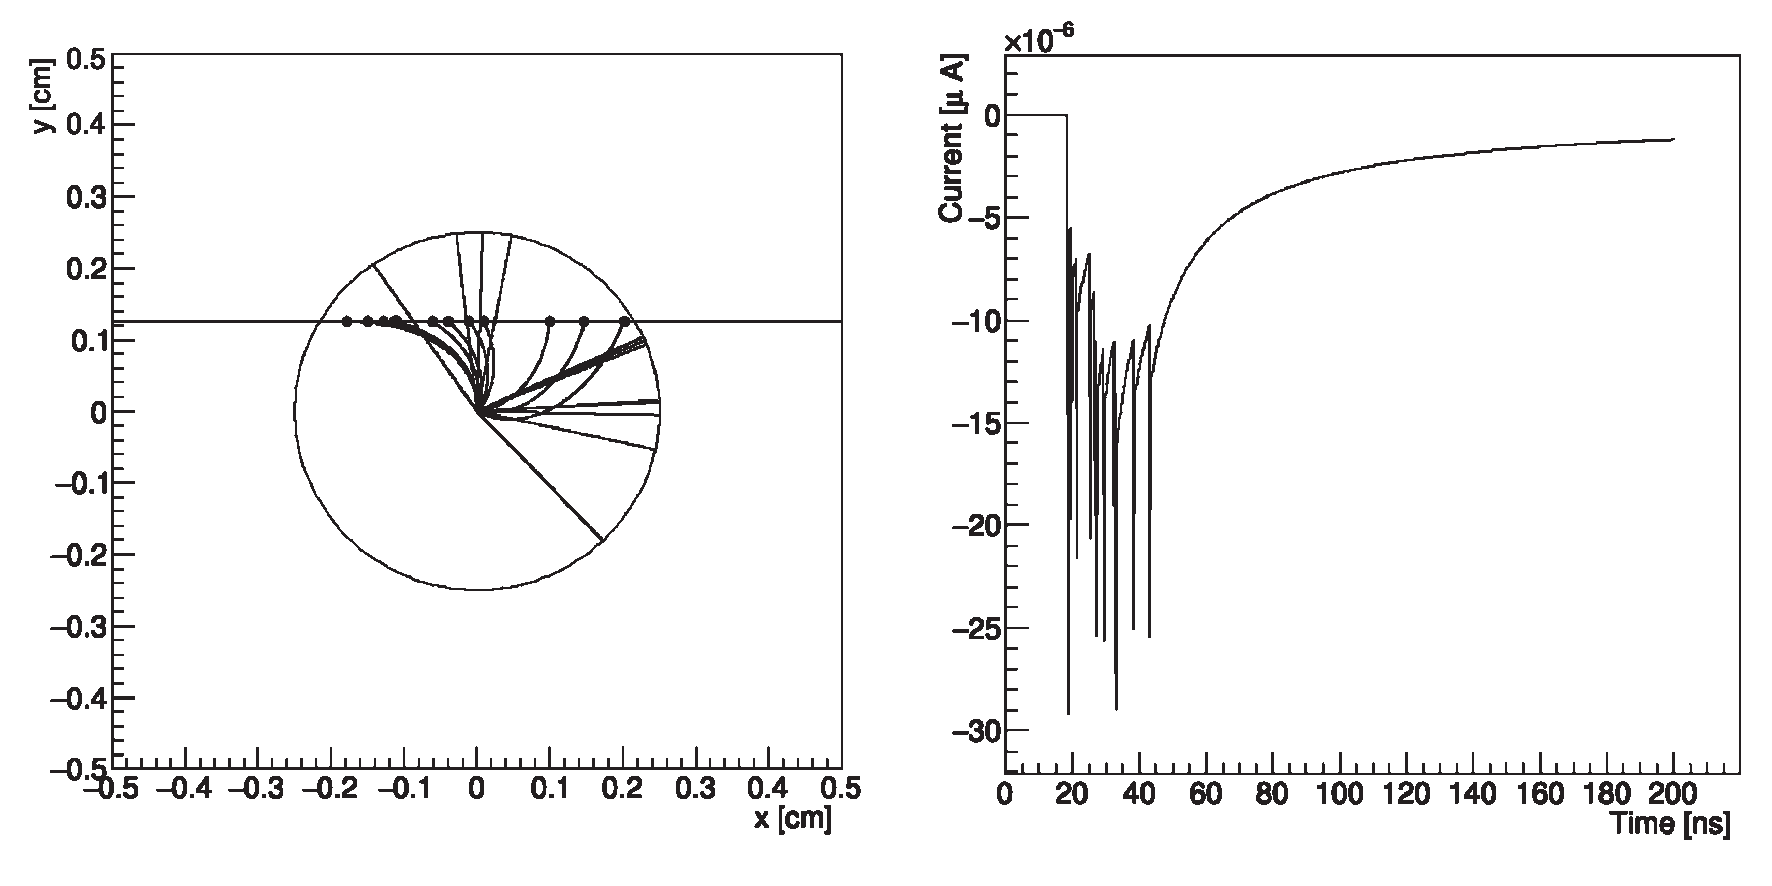
\includegraphics[scale=0.5]{Figures/StrawSignalGarfieldSim.pdf}
\decoRule
\caption{Left: Garfield simulation of the primary ionisations caused by a positron passing through the straw gas. Right: Garfield simulation of the signal measured from the sense wire for these primary ionisations.}
\label{fig:StrawSignalGarfieldSim}
\end{figure}
\fi
\section{Track formation}

The track fitting is required to work in the presence of pileup of multiple tracks at one time and include the uncertainty on the track position caused by the straw resolution. A charged particle travelling in a uniform magnetic field perpendicular to its motion will travel in a helical path. The tracking detectors are situated in the fringe field of the magnet and as such the particles experience a varying magnetic field radially and vertically. The radial field varies from 0 T at the outer end of the trackers to 0.3 T at the inner end. The vertical field also reduces to half of the 1.451 T storage ring magnetic field \cite{geanefitting}. This complicates the track fitting of the helical trajectory. This change in magnetic field will also effect the path of the charged particles as they drift through the straw, causing an added complication in obtaining the DCA for the positron. The track fitting is instead done by separating the path into short sections. 

Drift circles are created and centered around the wire, using the drift radius calculated from the drift time and the drift velocity. By comparing the neighbouring straw drift circles potential tangents can be found. To do this a line of best fit can be drawn from the shortest distance of each tangent between two drift circles.

The trajectory of the positrons path through the straw tracking detectors is calculated from the DCA of the positrons path through multiple straws, along with detailed information on the positions and orientations of the straws. The stages of track finding are as follows. For each tracking module the straw hits within a time period are grouped together. This time period is approximately 100 ns and these hits are grouped together to form a time island. Next there is spacial grouping of these hits. This is first done by grouping straw hits within the same view (U or V) in different layers if they are adjacent. These are referred to as clusters. The clusters for the U and V views for a single module are then group together to form seeds. The candidate positron tracks are formed by grouping together seeds in different modules based on which seeds are close in time and proximity to the previous one. Once straws have been identified as part of a potential track the $t_{d}$ is determined in order to calculate the drift distance for each straw. The simplified version in which a positron is travelling at normal incidence, a t0 value for a cluster with individual hit times of $t_A$ and $t_B$ is calculated using the equation

\begin{equation}
t_{0} = \frac{1}{2}((t_{A} + t_{B})-(d/v_{drift})),
\end{equation}
where d is the distance between the two wires and $v_{drift}$ is the drift velocity.

This allows a $t_{0}$ value to be calculated for each straw and hence the $t_{d}$ can be calculated in order to determine the DCA and then the drift cylinder of the positrons trajectory. This also allows the calculation of which side the positron came from which cannot be determined from a single straw. In order to determine the vertical direction the next cluster (with a different view) must be included, as these straws are orientated at a different angle. However this leads to a degeneracy when allowing for incident particles coming from any angle. The radial degeneracy of the DCA measurement means it is hard to determine which side of the wire the particle travelled, this is called the left-right ambiguity. Multiple track fitting is required to determine which set of left-right combinations gives the best fit. 

The track fitting is carried out using the GEANE (Geometry and Error Propagation) fitting algorithm \cite{geane}. This algorithm is configured to look up the field at small intervals throughout its path length to account for the varying magnetic field throughout the tracker module. The track fitting relies on only the hit information from the U or V layers. This fitting algorithm connects the DCA's determined in each of the straws it passed through in the tracking station. One can define a $\chi^{2}$ for a track by dividing the residuals of measured and predicted track parameters by their errors:

\begin{equation}
\chi^{2}= (\vec{p}-\vec{x})^{T}(\sigma^{-1})(\vec{p}-\vec{x}),
\end{equation}
\noindent
where $\vec{p}$ are the predicted track parameters given from the fit, $\vec{x}$ are the measured track parameters and $\sigma$ is the covariance matrix x of errors on the fitted parameters.

The Geant4 error propagation calculates the error matrices and predicted track parameters by starting off with guesses and then propagating the track parameters from these guesses. This is done by propagating the positrons by their average trajectories and splitting the steps into small enough sections. Meaning that a helical trajectory can be used in a magnetic field with a very small variation. Minimising the $\chi^{2}$ with respect to the track parameters leads to an improvement in the track fit \cite{geanefitting}. An example of a formed track candidate is shown in figure 5.5.

\begin{figure}[th]
\centering
\includegraphics[scale=1.4]{Figures/Track.png}
\decoRule
\caption{A plot showing an example of a track candidate.}
\label{fig:Track}
\end{figure}

\section{Track extrapolation}

The track parameters can be extrapolated back to the muon decay point or forwards to the calorimeter. The track information determined at its entry point into the tracking station is used in the extrapolation algorithm. This propagates the particles trajectory from the station entry point backwards through the changing magnetic field to the estimated muon decay position in the storage region. This information is used to observe the stored muon beam profile. This is problematic as there is no constant decay position and so this point has to be predicted by the extrapolation algorithm. This is taken to be the position of radial tangency, where the positrons momentum is tangential to the storage rings magic radius. 

The straw tracker station is situated directly upstream of a calorimeter to be able to extrapolate the tracks downstream to the calorimeter. The extrapolation downstream is used to estimate its hit position in the calorimeter. This can then be compared to what the calorimeter detected and act as a cross check between the two detectors. The data can also be used to determine if the two detectors are aligned correctly and also reduce pileup of hits detected in the calorimeter. Pileup is caused if two low energy positrons hit the same calorimeter crystal within its timing and spacial resolution and are counted as one high energy positron.

The extrapolation algorithm uses a Runge-Kutta Nystrom algorithm \cite{rungekutta1}\cite{rungekutta2}. 
This uses track parameters determined for the entry point and exit point of the tracking station to either extrapolate forwards to the calorimeters or backwards to the decay point. This must also take into account the changing magnetic field that is seen in the tracking station region (fringe field region) and the varying magnetic field to the muon storage region. This extrapolation is done in small steps in order to determine the magnetic field at each location of the particles trajectory and if the particle is likely to hit material. If this is the case then the particle will scatter, losing energy and altering its path. These particles will not be used in the precise analyses of the beam dynamics.

\section{Tracking quality cuts}

Quality cuts are applied to the data in order to reduce the tails observed in the tracking distributions and reduce the tracking uncertainties. Since the tracking detectors are not the primary detectors for this experiment, the track quality cuts were chosen to be fairly strict. They are optimised such that a small subset of tracks, representative of the whole sample, are as accurate as possible. This will need to be improved for track only analyses of the g-2 data (for example the EDM measurement), but is sufficient for the primary goal of measuring the beam dynamics. Effective quality cuts include having at least 12 straw hits required per track as a low number of hits leads to an increased error in determining the vertex position, removing tracks which have from start to finish more than 30$\%$ of layers without a hit, requiring that the track residual (measured - predicted) position is smaller than 0.5mm for any hit. Below in Table 5.2 is a summary of the quality cuts used in the tracking analysis.

\begin{table}[h!]
\begin{center}
 \begin{tabular}{||c | m{5cm}||} 
 \hline
 Parameter & Quality Cut \\ [0.5ex] 
 \hline\hline
 Non-failed track/vertex &  \\ 
 \hline
 No volumes hit & \\
 \hline
 Number of straw hits  & >= 12 \\ 
 \hline
 pValue & 5$\%$ \\ 
 \hline
 $\sigma_{y}$ and $\sigma_{r}$ & 0.5 < $\sigma_{y}$ 3.5 mm and 0.5 < $\sigma_{r}$ 5.0 mm\\
 \hline
 Track Entrance Point (at 1st module) & 60 < x < 150 mm and -40 < y < 40 mm \\
 \hline
Drift times & 0 < and < 70 ns \\ 
 \hline
 Track residuals & < 500 $\mu$m \\
 \hline
 Fraction of missed layers & < 30$\%$ \\ 
 \hline
 |U - V hits| & <= 4 \\ [1ex] 
 \hline
\end{tabular}
\caption{The quality cuts applied to the tracking detector data.}
\label{table:2}
\end{center}
\end{table}

\section{Readout electronics}

Once a signal has been produced on a sense wire two sets of electronics are used to convert the analog signal into a digital signal. These are the frontend electronics and the backend electronics. The frontend electronics are the boards which detect the wire signals and processes these into straw hits. A photograph of the frontend electronics is shown in figure 5.6. The backend electronics are the electronic boards used to interface the data from all the frontend boards and also synchronise the signals using the experimental clock information.

\subsection{Frontend electronics}

\begin{figure}[th]
\centering
\includegraphics[scale=0.4]{Figures/manifoldelectronics.pdf}
\decoRule
\caption{A photograph of the manifold frontend electronics showing the important components.}
\label{fig:manifoldelectronics}
\end{figure}

The frontend electronics consist of ASDQs (Amplifier Shaper Discriminator with charge (Q)) boards which are located inside the tracker manifolds and used to convert the analog signals from the sense wire to digital hits. This data is then sent to the TDC (Time to Digital Converter) boards which are contained in the box attached to the Snouts called the Frontend Low voltage Optical Box to BackEnd Readout (FLOBBER). The ASDQ boards are situated directly at the end of the sense wire and as such are the first electronics to process the wire signal. The ASDQ boards are connected directly into the manifolds via long pins to provide electrical connection, with every ASDQ boards connecting to 16 sense wires and so requires four ASDQ boards per manifold.

The ASDQ boards take several steps in converting the analog signal into a digital signal. These are amplification, signal shaping, baseline restoration and discrimination. The signal is shaped to smooth out the multiple small peaks that are created by the multiple primary ionisations produced by the charged particle travelling through the straw. This creates a single smooth peak for a single charged particle. Baseline restoration is used to remove the long signal tail that arises from the much slower ion signal. Doing this also ensures that primary ionisations from the next charged particle to pass through the straw are not consealed by the ion tail. Meaning the two signals can be easily distinguished, increasing the rate of signals that can be determined. The discriminator is used to register when the signal passes a threshold and recording the digital straw hit as being from the leading edge where the signal first crosses over the threshold to the trailing edge where the signal goes below the threshold. A diagram showing the step the ASDQ takes to convert the analog to digital signal is shown in figure 5.7.

\begin{figure}[th]
\centering
\includegraphics[scale=0.5]{Figures/asdqsignalpath.png}
\decoRule
\caption{A diagram displaying the steps the ASDQ carries out to convert an analog signal to a digital signal. (a) Multiple short signals are measured for each of the avalanches caused the the primary interactions of the positron with the straw gas. (b) The amplification and shaping of the short signals into one smooth signal. (c) The discriminator selects the data that passes above the threshold shown by the red line. The blue lines indicate the section of the signal that passes above this threshold. (d) The digital signal created for the leading and trailing edges of the smoothed out signal. The ion tail is not included in the diagram \cite{analogtodigital}}.
\label{fig:asdqsignalpath}
\end{figure}

The digital signals from the ASDQ boards are then sent to a TDC motherboard via flexicables. A straw tracking module contains two logic boards and four TDC motherboards. With each motherboard containing two TDC chips each of which connects to an ASDQ board. The electronics for the U layer is housed in the bottom manifold and the electronics for the V layer in the top manifold. The ASDQ digital signal information is carried via Low Voltage Digital Signal (LVDS) flexicable to a TDC board which is stored in the FLOBBER and holds the HV and logic boards (LB). The FLOBBER was designed to hold the electronics externally (outside the vacumm chamber) from the manifold as they do not need to be directly connected to the sense wires and makes it much easier to cool and gain access to these electronics. The TDC board time stamps the ASDQ signal to the precision of 625 ps by the use of the experiments 40 MHz clock. This information is sent to the backend electronics including the hit channel and time of the signal leading edge which is set as the hit time. The low and high voltage required for the tracking modules is supplied by a low voltage crate and a high voltage CAEN SY127 crate \cite{CAEN} located in a rack in the centre of the storage ring. 

\begin{figure}[th]
\centering
\includegraphics{Figures/daqdata}
\decoRule
\caption{The path of the straw hit data, clock and control signals through the frontend and backend electronics in the straw tracker readout system.}
\label{fig:daqdata}
\end{figure}

\begin{figure}[th]
\centering
\includegraphics[scale=0.8]{Figures/daqdatachain}
\decoRule
\caption{The hierarchy of frontend and backend boards and the numbers of each electronic boards used in the straw tracker readout system.}
\label{fig:daqdatachain}
\end{figure}

\subsection{Backend electronics}

The backend electronics include logic boards (LB), the FC7 and the AMC13. The two LBs per module are also located in the FLOBBER and provide an interface to the ASDQ-TDC pairs (1 LB per 4 pairs) used to supply clock and control signals to the TDC's and gather the information together into a single data block to be processed downstream in the FC7 and AMC13 boards. The LB consists of three external interfaces. A fibre-optic cable which connects to the higher level backend electronics to receive the external clock and control signals, the LV line supplying low voltage to the frontend electronic boards and a serial communication port to the slow control hardware. The fiber optic cables are required to send data over large distances very quickly and so the higher level backend electronics can be stored away from the trackers. These are placed in the centre of the ring away from the magnetic field storage region, allowing magnetic materials to be used.

Three FC7 $\mu$TCA advanced mezzanine cards (AMC) are located in the $\mu$TCA crate located at the centre of the storage ring, each connected to 16 LBs (one tracker stations worth). The FC7 is used to supply the clock and control signals for the LBs and collect a hit data block from all the LBs into a singular block using an event builder. The AMC13 board is the most downstream board which is also housed in the $\mu$TCA crate and collects together the hit data from the 3 FC7 boards as well as distributing the clock and control signals to the tracker modules. The AMC13 connects to a computer in the counting room via a Gigabit Ethernet (GbE) fiber in which the hit data blocks from the frontend boards can be saved to disk. Diagrams of the heirachy of the frontend and backend electronics are shown in figures 5.8 and 5.9.

\section{Choice of wire voltage}

Gain measurements were carried out to find the optimal operational wire voltage for the modules. The gain is the ratio of the final number of electrons detected by the straw wire to the number of electrons initially liberated in a gas. A high voltage on the straw wire will lead to a larger electric field strength and therefore electrons in the straw will have higher energies after collisions, leading to an increased likelihood of more ionisations. Therefore a larger signal is detected by the straw wire. However if the wire voltage is set too high the gas in the straw starts to breakdown with too many hits being detected by the wire. This amplifies the measurement of one charged particle leading to saturation of the electronics. If the voltage is too low, it will give a low electric field strength in the straw. Thus too few electrons will be liberated during collisions to produce a large enough signal in the wire. As the signal must be above the discriminator threshold of 200 mV, this would lead to loss of data recorded.

An optimal wire voltage must be found in between these two effects. This is the plateau region, where the best balance of high gas gain along with the minimum breakdown of gas is located. To determine the optimal wire voltage, the number of straw hits for various wire voltages was measured. This was carried out using a radioactive $Sr^{90}$ $\beta^-$ decay source with two types of gases; 80:20 $Ar:C0_{2}$ and 50:50 $Ar:C_{2}H_{6}$. As can be seen by figure 5.10 for the tracker straw gas using 50:50 $Ar:C_{2}H_{6}$ below 1200 V the gain is too low for straw events. With increasing voltage the gain increases and so does the number of hits recorded by the electronics. At a voltage of approximately 1550 V the number of hits recorded plateaus. This indicates that at this voltage approximately all of the beta particles travelling through the straw are detected by the wire as hits. This continues until the voltage reaches about 1700V. From there onwards the hit rate increases due to an increasing gain indicating the breakdown of the gas. This means that each beta particle will cause multiple hits to be recorded. Therefore the optimal voltage for the wire should lie on this plateau range, with a voltage of 1650V being chosen.

\begin{figure}[th]
\centering
\includegraphics[scale=0.8]{Figures/plateau}
\decoRule
\caption{A plateau scan plot showing the number of hits from a $Sr^{90}$ source with wire voltage for both 50:50 $Ar:C_{2}H_{6}$ and 80:20 $Ar:C0_{2}$. This shows that for $Ar:C_{2}H_{6}$ the plateau region is in the range of approximately 1550V - 1700V. Therefore the ideal wire voltage is within this range.}
\label{fig:plateau}
\end{figure}

\section{Data quality monitoring}

Data Quality Monitoring (DQM) is used to enable the monitoring of the tracking detectors performance in real time during data taking. This is used to monitor the trackers performance and looking for problems with the data that shifters can quickly identify and rectify. Examples of things that can be monitored in real time include the position and motion of the extrapolated beam, the number of hits per straw which is used to look for noisy or dead straw and any change in the drift time which could indicate a leak in the straw. The tracking detectors have performed extremely well during data taking periods and so far there has been no detector down time due to HV trips. 

The control of data aquisition (DAQ) for the experiment is controlled by the Maximally Integrated Data Acquisition System (MIDAS) software package. This is used to handle data from the frontend electronics, building events coming from various hardware/software locations and writing the data. This converts MIDAS data to ART data (the event processing framework used for the experiment) and allows for real time viewing of data taking via a web page. figures 5.11 - 5.13 show several tracking detector DQM web pages.

\begin{figure}[th]
\centering
\includegraphics[scale=0.3]{Figures/DQMoverview.jpeg}
\decoRule
\caption{A DQM page displaying tracking plots during data taking. Top right: showing the number of straw hits in both stations and each tracker module. Bottom right: The expected and measured straw hit drift time. Bottom left: The average number of hits per TDC for the last 20 events for both stations. Top left: Unpacking information.}
\label{fig:DQMoverview}
\end{figure}

\begin{figure}[th]
\centering
\includegraphics[scale=0.3]{Figures/DQMtracks.jpeg}
\decoRule
\caption{A DQM page showing near real time track candidates for 3 modules in station 1.}
\label{fig:DQMtracks}
\end{figure}

\begin{figure}[th]
\centering
\includegraphics[scale=0.3]{Figures/DQMhits.jpeg}
\decoRule
\caption{A DQM page displaying the number of hits in almost real time for the front two tracking modules of station 1.}
\label{fig:DQMhits}
\end{figure}

\section{Straw Tracker performance}

The data taking for the run 1 physics was during 23rd March - 7th July 2018. These tracking plots in figures 5.14 - 5.21 were created using a dataset during this run called the 60 hour data set which was taken during 19th - 23rd April 2018. 

Figure 5.14 shows the all straws hits in both stations and is the first plot looked at to determine if there are any problems with the straws. This includes checking that there are no dead channels and no stand out straws with substantially more hits, which indicates a noisy channel.

\begin{figure}[th]
\centering
\includegraphics[scale=0.5]{Figures/DigitChannelMap_.png}
\decoRule
\caption{A 3D graph displaying the number of hits in each straw for both tracking stations. The higher numbered straws are positioned closer to the storage ring and so more hits are recorded.}
\label{fig:DigitChannelMap_}
\end{figure}

Figure 5.15 displays the sum of all the drift times for each straw. The hit time for the straw is used to group straw hits together to form tracks. From this a $t_0$ value can be determined and using equation 5.1 the drift time is calculated.

\begin{figure}[th]
\centering
\includegraphics[scale=0.4]{Figures/StrawDriftTime_.png}
\decoRule
\caption{The straw drift time as measured during data taking by the tracking detectors.}
\label{fig:StrawDriftTime_}
\end{figure}

Figure 5.16 shows the track moment for all tracks. It is not a smooth peak as it includes certain regions where they cross over the thresholds of the quality cuts. Figure 5.17 displays the extrapolated tracks positions in the storage ring. Figure 5.18 shows the azimuthal muon beam spot.

\begin{figure}[th]
\centering
\includegraphics[scale=0.4]{Figures/hMomentum_.png}
\decoRule
\caption{The track momentum distribution measured for tracks by the tracking detectors.}
\label{fig:hMomentum_}
\end{figure}

\begin{figure}[th]
\centering
\includegraphics[scale=0.9]{Figures/trackextrap.png}
\decoRule
\caption{A top-down view of of the storage ring with the positions of the two tracking stations and the reconstructed decay positions of the positron tracks.}
\label{fig:trackextrap}
\end{figure}

\begin{figure}[th]
\centering
\includegraphics{Figures/beamposition.png}
\decoRule
\caption{The muon beam distribution reconstructed from all extrapolated tracks}
\label{fig:beamposition}
\end{figure}

Figure 5.19 is the radial position versus time of the tracks showing the coherent betatron oscillation of the stored muon beam. The radial position of the tracks is shown in figure 5.20. From this plot the radial distribution looks like its peak is at around 20 mm. However if you look at figure 5.19 you can see that the distribution bunches up around this value and the projection of this onto the x axis is what is displayed in figure 5.20. If you look at the CBO it can been seen that the peak is actually around 9 mm. The vertical position of the tracks is shown in figure 5.21 for completeness.

\begin{figure}[th]
\centering
\includegraphics[scale=0.9]{Figures/trackercbo.png}
\decoRule
\caption{The track reconstructed decay radial position versus time for all tracks measured by the tracking detectors.}
\label{fig:trackercbo}
\end{figure}

\begin{figure}[th]
\centering
\includegraphics[scale=0.4]{Figures/RadialPosition_.png}
\decoRule
\caption{Reconstructed decay radial position for measured tracks.}
\label{fig:RadialPosition_}
\end{figure}

\begin{figure}[th]
\centering
\includegraphics[scale=0.4]{Figures/VerticalPosition_.png}
\decoRule
\caption{Reconstructed decay vertical position for measured tracks.}
\label{fig:VerticalPosition_}
\end{figure}

More details of the beam dynamics results will be given in chapter 7. The following chapter will provide details on the construction of the straw tracking modules. These results would not be possible if the tracking detectors were not made to very high specifications, which the following chapter will discuss in detail.



 
% Chapter 5

\chapter{Construction of the Straw Tracking detectors} % Main chapter title

\label{Chapter5} % For referencing the chapter elsewhere, use \ref{Chapter5} 

\section{Introduction}

This chapter will give details on the construction of the E989 straw tracking detectors as described in Chapter 5. This includes each step in the construction process and the strict quality control tests which were meticulously carried out after each of these steps. This was done to ensure that the tracker modules run effectively and meet the design specifications required by the Technical Design Report (TDR)\cite{Reference29}.

The straw tracking detectors were constructed by University of Liverpool staff and students in the ISO Class 5 cleanroom. This was done to prevent any contaminants from entering the module during construction. A total of 22 modules were produced and tested in Liverpool before being shipped to Fermilab. 

\section{Pre-assembly checks and preparation}

Before construction can be started a series of checks and preparations must be carried out prior to beginning construction of a tracking module. The gold-plated copper pins which fix the wire in place within the manifold must be cleaned for any blockages inside before they can be used to construct wires. This is done by placing the pins in an ultrasonic cleaner which uses de-ionized water and then secondly cleaned with isopropanol alcohol. Once the pins have dried, any remaining blockages can be removed by threading the pins with thicker 50 $\mu$m gold-plated tungsten wire. The Aluminized Mylar straws are also visually inspected for any observable damage, kinks or unravelling of the straws that would lead to gas leakage. These straws are not passed onto the next stage of construction. 

The straws are measured and should all be approximately 1.3 m long and 5 mm in diameter. The electrical resistance is measured before and after the supportive inner layer of paper is removed from the straw. If the resistance changes dramatically after the removal of the paper, this would indicate that damage has been created when removing it. The resistance for each straw should be around 200$\Omega$ for both measurements. Any straw with a much higher or lower value or a straw with a changing resistance will not be used in the construction process. The straws that pass will then be prepared for a leak test. 

\subsection {Leak testing}

The rate of permeation of $CO_{2}$ that flows through the straw wall is calculated for every straw. Only the straws with the lowest permeation rates and do not exceed the leak rate specified by the TDR will be selected for module construction. As the Mylar straws are known to be permeable to some gases it was predicted that some gas leakage would be present. The experiment is operated under vacuum and in order for the quadrupoles to operate at the required voltage the Storage Ring vacuum cannot exceed $10^{-6}$ Torr. In order to achieve this each tracker station must have a maximum leak rate of $4.5\times10^{-5}$ Torr·L/s, therefore each tracking module must not exceed $5.6\times10^{-6}$ Torr·L/s. Anything above this is too high to be handled by the Storage Ring pumping system.

\begin{figure}[ht]
\centering
\includegraphics[scale=0.8]{Figures/leaktestsetup}
\decoRule
\caption{Photograph of a straw being placed into the leak testing equipment.}
\label{fig:leaktestsetup}
\end{figure}

The leak tests were done using $CO_{2}$ rather than the experimental gas mixture of 50:50 $Ar:C_{2}H_{6}$ as this was not available for use in the University of Liverpool cleanroom. The leak rate measured is then converted to $Ar:C_{2}H_{6}$ to determine if the straws have a low enough permeation rate to be used in the experiment. The chamber for testing the permeation rate is constructed from Copper pipes and was designed by members of the Mu2e experiment. A photograph of the setup is shown in figure~\ref{fig:leaktestsetup}. This chamber will hold a Nitrogen environment while a straw is placed inside and includes a $CO_{2}$ sensor. The method of the leak testing begins by flushing the test chamber with Nitrogen to remove any other gases present in the chamber. Whilst this is taking place the straws are flushed with $CO_{2}$ to clear out any other gases within the straws. This is done by gluing a gas inlet of Viton tubing to each end of the straw. The gas line to the $CO_{2}$ is then attached to one end to flow the gas through the straw. This is done for one minute. Then the end furthest from the gas line is sealed to allow the straw to fill up with $CO_{2}$. Initially this is over pressured to 1.7 relative to Atm. This is to ensure that the straws will easily be able to cope with the experimental vacuum of 1 Atm. The gas pressure is then reduced to 1 Atm relative and filled at a rate of 0.15 LPM. While this is occurring the straw is inspected for any leaks. The straw is then sealed off from the flow of $CO_{2}$ and further inspected for any deflation of the straw due to holes. The straw is then immediately placed into the test chamber which is then sealed shut. Ensuring that the straw is not kinked or bent at all throughout the testing process to minimise the risk of damage to the straw. Within the test chamber, the $CO_{2}$ sensor records the levels of $CO_{2}$ that passes through the straw wall into the test chamber. This test is carried out for 40 minutes with the $CO_{2}$ level as a function of time displayed. The leak rate is calculated as a slope of this distribution as shown in figure~\ref{fig:leaktestplot}. There were two separate batches of straws tested throughout the construction process. During pre-testing preparation it was discovered that the PPG4 straws had a wall thickness of 13$\mu$m, which is 2$\mu$m less than batch PPG3. Due to the concern that the PPG4 straws would have a much larger permeation rate and therefore a larger failure rate studies were carried out to see if the maximum leak rate for the PPG4 straws could be increased and still be under the required leak rate. To keep within design specifications the final leak rates allowed were a maximum leak rate of $20\times10^{-5}$cc/min for the PPG3 straws and $40\times10^{-5}$cc/min for the PPG4 straws. The pass rates for all PPG3 straws was 88$\%$ and 86$\%$ for all PPG4 straws.

\begin{figure}[ht]
\centering
\includegraphics[scale=0.62]{Figures/leaktestplot}
\decoRule
\caption{Graph of a straw with a passed leak rate of $4.83\times10^{-5}cc/min$.}
\label{fig:leaktestplot}
\end{figure}

\subsection {Pre-installation ASDQ testing}

Prior to installation each ASDQ board was tested to ensure that the readout electronics and all 16 channels per ASDQ board were working correctly. This involves a setup where each ASDQ is connected by Kapton flexi-cables to a set of  secondary electronics as would be done in the actual experimental setup, shown in figure~\ref{fig:ASDQtestSetup}. Instead of using muon cosmic data which is used in a later stage of module testing, pulses are sent to the ASDQ. Here 20 pulses are sent to each of the ASDQ’s 16 channels, where the leading edge and the trailing edge are counted. If the channel is working correctly all the pulses should be sent back and so 40 hits will be read per channel. A plot of an ASQD working correctly is shown in figure~\ref{fig:asdq_testing1}. An example of an ASDQ with connection problems is shown in figure~\ref{fig:asdq_testing2}. Out of 165 ASDQs tested, 24 failed giving a pass rate of 85.5$\%$.

\begin{figure}[ht]
\centering
\includegraphics[scale=0.3]{Figures/ASDQtestSetup}
\decoRule
\caption{Photograph of testing two ASDQ boards with the ASDQ testing setup.}
\label{fig:ASDQtestSetup}
\end{figure}

\newpage
\vfill
\begin{figure}[ht]
\centering
\includegraphics[scale=0.48]{Figures/asdq_testing1}
\decoRule
\caption{Example plot of an ASDQ that has passed testing with all channels recording 40 hits.}
\label{fig:asdq_testing1}
\end{figure}

\begin{figure}[ht]
\centering
\includegraphics[scale=0.48]{Figures/asdq_testing2}
\decoRule
\caption{Example plot of an ASDQ that has failed testing. This shows that there are several noisy channels producing more than 40 hits.}
\label{fig:asdq_testing2}
\end{figure}
\vfill
\clearpage

\section{Metrology}

Before assembly, the manifolds, flanges and lids are metrology tested. This is to determine the flatness, any tilts of the pieces, along with any wrongly sized or positioned holes. The information is also used to match together two manifolds and a flange for every module. 

\begin{figure}[ht]
\centering
\includegraphics[scale=0.3]{Figures/Flangedrawing.pdf}
\decoRule
\caption{Engineering drawing of the flange with the nominal hole positions and sizes displayed.}
\label{fig:Flangedrawing}
\end{figure}

After the manifolds, flanges and lids have been machined the dimensions of various features of the manifold including dowel holes, surfaces and the size and position of each straw hole is precisely measured using a contact probe with a Coordinate Measuring Machine (CMM). The aim is to learn how accurately the parts have been machined and hence to assess if they lie within acceptable tolerances. Therefore determining whether they are ready for use in module construction or need to be returned to the workshop for alteration. An engineering design sheet showing the required hole positions and sizes for the flange is shown in figure~\ref{fig:Flangedrawing}. The dimensions of each piece are required to be known accurately for alignment of the tracking detectors once they are placed into the storage ring. A program was written to measure these points automatically as previously all 1326 points needed for the measurements were done by hand. This improved the measurement time from approximately 6 hours manually to 50 minutes automatically. The manifolds are then paired with a vacuum flange based on the offsets also measured in the flanges. The data is stored in the Liverpool construction database which could then be utilised for any detector alignment studies required.

\begin{figure}[ht]
\centering
\includegraphics[scale=1.3]{Figures/cmm1}
\decoRule
\caption{Picture of a CMM measurement of the manifold straw holes.}
\label{fig:cmm1}
\end{figure}

The software Metrosoft Quartis \cite{metrosoft} was used to write a program to control the CMM to measure all the parts of the manifold, flange and lid required. This program uses CAD models of the modules pieces to select the elements to assess and the number of probe points required for each measurement. A separate program was written to measure the all three pieces.

The manifold is glued to a stand which is itself fixed in position to the granite work surface of the CMM. This ensures the position of the piece relative to the granite work surface is constant for each separate manifold measurement. Therefore the probe can find the correct position to start its measurement program. The setup is shown in figure~\ref{fig:cmm1}. From this a coordinate system for the stand can be set up and used each time so that the probe will automatically know where it is relative to the manifold. This is done using the 3-2-1 method. Where manually a plane of 3 points is made on the stands face. This is set to a primary direction of z and origin of z. Next a line of two points is measured on the side face of the stand, setting a secondary direction of x and an origin of y. A point is then measured on the other face and set as the origin of x. This was done the first time a program was written, saved and used each time. Next the manifold coordinate system is created with its origin located on a corner of the manifold end. This is done using the 3-2-1 method again. This co-ordinate system is shown in figure~\ref{fig:cmm2}. This coordinate system is saved and will be redone each time a new manifold is measured as there is likely to be a slight deviation in the position compared to the previous manifold measured. This ensures the coordinate system of the CAD is updated to the correct alignment for each metrology measurement. 

\begin{figure}[ht]
\centering
\includegraphics{Figures/cmm2}
\decoRule
\caption{Setup co-ordinate system of the manifold.}
\label{fig:cmm2}
\end{figure}

\begin{figure}[ht]
\centering
\includegraphics[scale=0.5]{Figures/ccmprogram.png}
\decoRule
\caption{Left: A screenshot of the Metrosoft Quartis program. Right: A screenshot of the program display as the CMM program is running to measure the manifold.}
\label{fig:cmmprogram}
\end{figure}

\begin{figure}[ht]
\centering
\includegraphics[scale=0.35]{Figures/cmmresults.png}
\decoRule
\caption{Graphical images of results from the Metrosoft Quartis database. Left: A plot of a dowel hole displaying the probes points and their difference from their nominal value. Right: A plot of a plane on the manifold with the probe points showing their difference from the nominal flatness in mm.}
\label{fig:cmmresults}
\end{figure}

At the start of a new set of measurements the probe dimensions needed to be calibrated manually using the reference sphere. The dowel holes and 128 straws holes of the manifold are required to be known in size and position precisely. These were measured as cylinders by the probe which could also determine if there were any bumps inside the holes which would need to be removed. The programming of the measurement of the dowel holes and straw holes is shown in figure~\ref{fig:cmmprogram}. The straw hole measurements were carried out by a program using a loop which measures a cylinder and moves the probe 6.052 mm along to the centre of the neighbouring hole. This was done for each straw row. As the expected positions are given in the CAD model any deviations of individual holes or offsets of entire rows will be measured by the probe. Along with the holes, the various manifold faces and O-ring plane were also measured for flatness, tilting and positioning.

Once all measurements are completed, the database contains all the values required including nominal values, the values measured and the range of measurements for each element. From this data any alterations to the pieces of equipment can be carried out. The data is then used to match pairs of manifolds together with similar offsets and chose a flange to match with the manifolds. Plots from the database showing a cylinder from a dowel hole measurement and a surface element from a manifold surface displaying the measured probe points deviation from the nominal values are shown in figure~\ref{fig:cmmresults}. Plots showing the straw holes and flange dowel holes measured are shown in figures~\ref{fig:strawholesizes} and~\ref{fig:dowelholesizes} respectively.
%put in a histogram of the hole sizes (difference from nominal) and positions (difference from nominal)

\begin{figure}[ht]
\centering 
\includegraphics[scale=0.6]{Figures/strawholesizes.jpeg}
\decoRule
\caption{Plot displaying the measured manifold straw hole sizes for all manifolds measured. The nominal size for a straw hole being 5.15$\pm0.2$ mm. }
\label{fig:strawholesizes}
\end{figure}

\begin{figure}[ht]
\centering 
\includegraphics[scale=0.6]{Figures/dowelholesizes.jpeg}
\decoRule
\caption{Plot showing the size of all flange dowel holes measured. The nominal size for a flange dowel hole is 5.0$\pm0.2$ mm.}
\label{fig:dowelholesizes}
\end{figure}

\section{Preparation of wires (Wire crimping and threading)}

The wires are prepared prior to being strung into the manifold. This involves threading the wire through gold plated Copper pins. The 25 $\mu$m gold plated Tungsten wire is threaded through a long pin which is then crimped using the materials tester to secure the wire in place. The copper wire must be cut to a length longer than the straw module, so lengths of about 80cm were cut. The wire is threaded through the injection molded insert which contain slots to allow gas flow through the straws and secondly through a long pin. Glue is then applied to the end of the long pin which is then placed inside the insert, leaving a small length of the wire going through the pin with most left behind the insert. 

To secure the wire in place the long pins are crimped using a Lloyd LRX Plus materials tester \cite{LloydPlus}. The pins are placed horizontally into the materials tester to ensure an even distribution and are crushed using a 1kN load cell. A photograph of the crushing process is shown in figure~\ref{fig:crimpmachine} with a close up photograph shown in figure~\ref{fig:pincrush}. To measure this process a Epsilon Extensionometer \cite{Extensionometer} is attached to the crushing jaws to measure its extension as it crushes the pin. This data produces a graph which is checked to ensure that the crimping was carried out correctly, along with the measurement of the pins diameter before and after crimping.

The wires are then left for 24 hours to allow for any expansion of the pin after the crimping process. The short length of the wire is then gently pulled while holding the insert to see if the wire can be pulled through and hence the crimp has failed. Any wires that fail this will be re-crimped and pull tested again. 

\begin{figure}[ht]
\centering 
\includegraphics[scale=0.70]{Figures/crimpmachine}
\decoRule
\caption{Photograph of the Lloyd LRXPlus materials tester crimping a pin.}
\label{fig:crimpmachine}
\end{figure}

\begin{figure}[ht]
\centering 
\includegraphics[scale=0.08]{Figures/pincrush.jpg}
\decoRule
\caption{Close up photograph of a pin being crushed.}
\label{fig:pincrush}
\end{figure}

\section{Straw assembly}
The long straws that have passed leak and resistance tests are then cut into 90.6 mm sections with a guillotine. This usually makes 12 shorter straws. The top hat and non-top hat end pieces are then glued to each end of the straw. This is done using a Q-tip to carefully apply a silver epoxy TraDuct 2902 \cite{silverepoxy} to the end pieces and attach them to the straw ends ensuring that the straws are not bent or damaged as the two are bonded together. A row of completed straws is shown in figure~\ref{fig:completestraws}.

\begin{figure}[ht]
\centering 
\includegraphics[scale=0.05]{Figures/completestraws.jpg}
\decoRule
\caption{Photograph of a row of 32 completed straws.}
\label{fig:completestraws}
\end{figure}

The selected manifold pair plus the flange are put together, positioned correctly and then secured in place by jacks which hold the manifolds a selected distance apart. Then the module is potted with 128 straws. In total the process to glue 128 straws into the module takes 5 days. Firstly the straws have silver epoxy applied between the straw and module. This is used to produce an electrical grounding of the straw to the module. To provide a gas seal between the straw and the module Araldite 2020 is also applied. The process requires 5 days due to the time that the curing takes to dry and the fact that only one layer is done at a time to minimise the risks of moving or knocking the straws while the bond is curing.

\section{Module construction}

The modules are placed on the stringing jig which is used to populate the straws with the individual wires. The prepared wire is threaded through a straw using a plastic rod with a hole in the end to attach the wire. This will be pulled the entire way through a straw to the opposite end and removed from the other side to thread the wire. A photograph of this is shown in figure~\ref{fig:string}. The end with the pre-crimped pin goes into the top hat side of the straw and is fixed there while the bare end of the wire is pulled through to the other end of the straw. Another insert is threaded through the wire and fixed into the non-top hat end, with a short annealed pin being threaded onto the wire. The short pin is annealed so that it is easier to crimp with a hand tool. Once both the insert and pin are threaded through the wire a 30 g weight is hung from the end of the wire to provide the required tension while the pin and insert are being secured into the module and until the wire has been crimped and fixed in place. The short pin is then glued into the insert and then the pin is crimped with a hand crimp tool to secure the wire in place. The remaining wire with the weight attached is then cut off and the wire trimmed off as close as possible to the pin end. Glue is then placed on top of the wire to cover it and stop any electrical discharge that could occur. The stringing process is repeated for all 128 straws. Once the stringing process has been completed, the jacks that are holding the manifolds in place are moved apart 50$\mu$m to produce a 50 g tension equally to the straws and wires. This is done to compensate for expansion under vacuum.

\begin{figure}[ht]
\centering
\includegraphics[scale=0.80]{Figures/string}
\decoRule
\caption{Photograph of a wire being threaded into a straw on the stringing jig.}
\label{fig:string}
\end{figure}

\section{Post module assembly wire testing}

The wires are required to have a tension test after stretching to ensure that no wire failures have occurred. A tension within 25-50g is required, preferably the wires being closer to 50g. This is about half of the tension needed to break a wire. The higher tensions are desirable to minimise the gravitational sag on the wires.

The tension test is carried out by placing a magnet above the test straw. This is positioned above the straw onto a thin layer of perspex to protect the straws. Crocodile clips connecting to the tension tester are attached to each end of the straw pins. The tension is measured by sending current down the wire and varying its frequency in an external magnetic field. The varying electric field will induce a magnetic field and cause the wire to resonate in the external magnetic field. The current of the wire is recorded after every pulse. When the frequency of the current pulse reaches the resonance frequency of the wire, the current induced in the wire will be recorded and used to calculate the tension. A photograph of a tension test is shown in figure~\ref{fig:wiretesting}.

The tension tester calculates the wire tension using the equation: 
\begin{equation}
f=\frac{\sqrt[2]{\frac{T}{\frac{m}{L}}}}{2L}
\end{equation}
where f is the frequency in Hertz, T is the tension in Newtons, m is the mass of the wire in kilograms and L is the length of the wire in metres. 

\begin{figure}[ht]
\centering 
\includegraphics[scale=0.07]{Figures/wiretesting.jpg}
\decoRule
\caption{Photograph of a tension test being carried out on a wire.}
\label{fig:wiretesting}
\end{figure}

A resistance test is also carried out on each wire. This is done by touching probes to the pins on either end of the wire which are connected to a digital multimeter. The resistance of each wire should be within the range of 10 - 13 $\Omega$. If wires lie outside this range, they will be removed and re-strung. A carbon fibre post is then fitted the non flange end of the module and used to keep the manifolds in position. The new manifold separation distance is checked using the CMM, and then the jacks can be removed.

\section{Module electronics installation}

Once the resistance and tension tests have been completed with any re-stringing done and the wires have passed all requirements the modules electronics can be inserted. The electronics required include eight ASDQ boards (four per manifold) which are placed onto readout long pins. End caps are placed onto the short pins providing insulation to stop any electrical discharge from the pin to the ASDQ boards. The two ASDQ chips on each board are then covered with a PTFE thermal heat pad. This is to prevent the boards overheating by transferring the heat to Copper heat sinks which are fixed to the ASDQ boards using brass screws. The heat sinks pass the heat onto the manifold. Four flexi cables and HV cables are connected to the feedthrough board and inserted through the Snout and connected to the relevant ASDQ boards. A photograph of this is shown in figure~\ref{fig:flexicables}. The feedthrough board is then fixed to the Snout and sealed up to provide a gas seal. Finally the o-ring is covered in vacuum grease, put in place then the lid is secured in position with a torque wrench to seal the lid to the manifold and ensure the lid is attached evenly.

\begin{figure}[ht]
\centering
\includegraphics[scale=0.4]{Figures/flexicables}
\decoRule
\caption{Photograph of flexi cables and HV internal cables connected to the feedthrough board at Snout end of the module.}
\label{fig:flexicables}
\end{figure}

\section{Module Checks and Data Quality}

Before the constructed modules can be shipped to Fermilab, several tests must be carried out to ensure that the module can run at a sufficient vacuum, all wires are recording hits correctly and that the module can run at the required high voltage for a sufficient amount of time. These tests are done by placing the module horizontally into a vacuum chamber to provide the maximum number of cosmic hits for data taking. The module is bolted into the vacuum tank and vacuum sealed using a greased O-ring. The 80:20 Ar:$CO_2$ test gas is flowed through the module at a rate of 0.1LPM into the top manifold, out through the bottom manifold and directed into a bubbler. This is used to check the gas flow. A photograph of the setup is shown in figure~\ref{fig:DAQsetup1}.

\begin{figure}[ht]
\centering
\includegraphics[scale=0.4]{Figures/DAQsetup1}
\decoRule
\caption{Clean room setup for module testing including the vacuum tank for vacuum testing on the left and CAEN power supply on the right.}
\label{fig:DAQsetup1}
\end{figure}

\subsection{Vacuum testing}

The vacumm pump down begins with a roughing pump which takes it down to 10 mbar. Then the turbo pump is needed to lower the pressure to the order of $10^{-6}$ mbar as required for the experiment. This data is continually monitored as shown in figure~\ref{fig:vactankpressure}. If the module pressure struggles to get below $10^{-3}$ mbar after one day of pumping, this indicates that the module has a leak that needs to be investigated. The vacuum will be monitored to ensure that the pressure can stay to the required level for significant amount of time.

\begin{figure}[ht]
\centering
\includegraphics[scale=0.4]{Figures/vactankpressure}
\decoRule
\caption{Graph of a successful module pump down, with rapid pump down on the left and vacuum shut down on the right.}
\label{fig:vactankpressure}
\end{figure}

\subsection{ High and low voltage noise scans}

Once the required vacuum level has been maintained the Front End Electrons as explained in chapter 5 are placed into a custom made box which is fixed to the Snout. Low and high voltage noise scans will be carried out to ensure that no residual noise from the wires is observed above the 200mV threshold. This also checks if all the connections to the internal electronics are working, with the 16 channels per ASDQ board all recording data. If channels are not working this could indicate a shorted connection, a broken wire or problems with the HV connection. The threshold was set at 200mV as this was deemed high enough to cover most of the residual noise from the wires whilst not losing too many low energy straw hit signals. For noise scans every channel is tested at three voltages of 1000V, 1250V and the near-operating voltage of 1500V. The actual voltage in the experiment is 1650V, but Ar:$CO_2$ breaksdown at this value, and could contaminate the wires. If working correctly all the channels at all voltages should be working identically. A plot of an ASDQ that passed a noise scan is shown in figure~\ref{fig:HighVNoiseScans}. For channels that do not work, this would show that the wire connection is faulty or that the wire has a contaminant. Once 1500V has been successfully reached, this is left for a day to test if it runs stably. If a failure is observed and it is suspected to be due to a wire contaminant then high voltage training is carried out. To do this the HV is increased in increments of 100 V from zero until the channel trips. Then the trip current is increased from 1$\mu$A to 3$\mu$A and left at this current for a couple of hours to remove the contaminant.

\begin{figure}[ht]
\centering
\includegraphics[scale=0.8]{Figures/HighVNoiseScans}
\decoRule
\caption{Example plot of a High voltage noise scan that has passed testing.}
\label{fig:HighVNoiseScans}
\end{figure}

\subsection{ Module testing using cosmic muon data}

Once all testing has been completed and the vacuum and HV are running stably then DAQ runs with muon cosmic data are taken. A four hour test, which is the minimum time required to detect hits in all 128 channels, was carried out. If a channel had zero hits in this time it indicates a dead channel. Once any dead channels have been fixed much longer cosmic data runs were carried out. This was to ensure that the module could record data stably for a significant amount of time. Plots of a long cosmic run are shown in figures~\ref{fig:cosmicdata1} and~\ref{fig:cosmic4rows} displaying the hits recorded in all four rows of straws.

\begin{figure}[ht]
\centering
\includegraphics[scale=0.65]{Figures/cosmicdata1}
\decoRule
\caption{A plot of cosmic data channel hits for the four rows of straws.}
\label{fig:cosmicdata1}
\end{figure}

\begin{figure}[ht]
\centering
\includegraphics[scale=0.4]{Figures/cosmic4rows.png}
\decoRule
\caption{A 3D plot showing more clearly the cosmic data channel hits for the four rows of straws.}
\label{fig:cosmic4rows}
\end{figure}

Once it has been established that the module has passed all quality assurance testing the module is readied for shipping to Fermilab. This involves covering the module with perspex shielding and an antistatic plastic covering before being placed into a pelicase.


 

\chapter{Vertical betatron oscillations} % Main chapter title
\label{Chapter6} % For referencing the chapter elsewhere, use \ref{Chapter6} 

\section{Introduction}

The muon g-2 storage ring acts as a weak focusing betatron. The experiment uses quadrupoles held at an adjustable voltage. The electric field provided by the quadrupoles gives a linear restoring force in the vertical direction, focusing the beam vertically but defocusing radially. However, the combination of the vertical dipole magnetic field and the defocusing radial electric field provides a net linear restoring force in the radial direction and so the beam is focused in both directions. The E-field and the B-field determine the dispersion of the beam and the $\beta$-functions, the measurements of which will be the focus of this chapter.

The muons that enter the ring have to pass through the inflector, which is an aperture vertically $\sim{15}$ cm and radially $\sim{7}$ cm wide. These muons do not all have the magic momentum and so the beam has a momentum spread. The restoring forces from the two fields cause the muons to oscillate about an equilibrium position. Vertically, for ideal quadrupoles, the equilibrium position $y_{e}$ is at the centre of the storage ring $(y = 0)$. The radial equilibrium position $x_{e}$ is determined by the muons momenta. This leads to both the average position and width of the muon beam to exhibit simple harmonic motion called betatron oscillations, in both the radial and vertical directions. 

The equations for the horizontal and vertical beam motion are given by 
\begin{equation}
x = x_{e} + A_{x}\mathrm{cos}(v_{x}\frac{s}{R_{0}} + \delta_{x}),
\end{equation}
\begin{equation}
y = y_{e} + A_{y}cos(v_{y}\frac{s}{R_{0}} + \delta_{y}),
\end{equation}

\noindent
where $\nu_{x}$ and $\nu_{y}$ are the horizontal and radial beam tunes respectively, s is the arc length along the trajectory, $R_{0}$ is the magic radius and $\delta_{x}$ and $\delta_{y}$ are the corresponding phases. The tune is defined to be the number of betatron oscillations per revolution of the storage ring and is related to the strength of the field, characterised by the field index n. The field index is given by:

\begin{equation}
n=\frac{{\kappa}R_{0}}{{\beta}B_{0}}
\end{equation}

\noindent
where $\kappa$ is the electric quadrupole gradient, $R_{0}$ = 7112mm which is the radius of the storage ring, $\beta$ is the relativistic velocity of the muon and $B_{0}$ is the magnetic field strength. The corresponding tunes are:

\begin{equation}
v_{x} = {\sqrt{1-n}},
\end{equation}
\begin{equation}
v_{y} = \sqrt{n}.
\end{equation}

To go from the tunes to the oscillation frequencies we multiply by the cyclotron frequency $f_{c}$. For the initial running conditions the quadrupoles were set to $18.3$ kV during data taking, giving a corresponding field index of $n = 0.108$. The resulting horizontal and vertical betatron frequencies are:

\begin{equation}
{f_{x} = f_{c}\sqrt{1-n} \simeq 0.94f_{c}} = 6298\mathrm{ kHz},
\end{equation}
\begin{equation}
{f_{y} = f_{c}\sqrt{n} \simeq 0.33f_{c}} = 2211\mathrm{ kHz}.
\end{equation}

\subsection{The effect of betatron oscillations on $\omega_{a}$}

Precise knowledge of the muon beam distribution and its behaviour throughout the fill is required to determine the corrections needed to calculate $a_{\mu}$. This is because as the beam undergoes these radial and vertical oscillations the rate of positrons measured by the detectors, which have an acceptance that depends upon the decay position, also oscillates. Thus the total number of detected positrons will vary throughout the fill due to the oscillation of the centroid of the beam distribution, as well as due to the precession of the muon spin and the width. The simple 5 parameter fit function used to fit $\omega_{a}$ is 

\begin{equation}
N(t)_{5par} = N_{0}e^{-\frac{t}{\gamma\tau}}(1+A\mathrm{cos}(\omega_{a}t + \phi))
\end{equation}

\noindent 
Where $N_{0}$ is an estimate of the number of muons at start time, $\gamma\tau$ is the average relativistic lifetime of the stored muons, A is the amplitude of the precession oscillation (asymmetry term) and $\phi$ is the phase of precession at the start time. This is modified to account for the variation in the positron rate due to the betatron oscillations by:

\begin{equation}
N(t) = N(t)_{5par}\cdot{N_{CBO}}(t),
\end{equation}
\noindent
with
\begin{equation}
{N_{CBO}}(t) = 1 + A_{CBO}\mathrm{cos}(\omega_{CBO}t) + \phi_{CBO})e^{-\frac{t}{\tau_{CBO}}}
\end{equation}

\noindent
Where $A_{CBO}$ is the amplitude of the CBO, $\omega_{CBO}$ is the frequency of the CBO term, $\phi_{CBO}$ is the phase of the CBO at the start time and $\tau_{CBO}$ is the lifetime of the CBO. The general form for an oscillation term is an exponentially decaying sinusoid. One such term is added for all the observed betatron oscillations. As well as directly affecting N, there are effects from the betatron oscillations on the phase and amplitude in the final $\omega_{a}$ fits. 

\begin{equation}
{A}(t) = 1 + A_{A}\mathrm{cos}(\omega_{CBO}t + \phi_{A})e^{-{\frac{t}{\tau_{CBO}}}}
\end{equation}

\begin{equation}
{\phi}(t) = 1 + A_{\phi}\mathrm{cos}(\omega_{CBO}t + \phi_{\phi})e^{-{\frac{t}{\tau_{CBO}}}}
\end{equation}

\noindent
Here we have moved from A and $\phi$ defined in equation 7.8 to time dependant A and $\phi$, where $A_{A}$ and $\phi_{A}$ refer to the amplitude and phase of the CBO oscillation in the asymmetry term and $A_{\phi}$ and $\phi_{\phi}$ are the amplitude and phase of the CBO oscillation of the $\phi$ term. The relevant betatron oscillations for the run 1 dataset are defined later in this chapter. In order to minimise the impact of these oscillations on the $a_{\mu}$ measurement tuning is required in order to ensure that the betatron wavelengths are not multiples of the storage ring circumference. If the beam after one full rotation around the ring is situated back in the same exact position then the beam would sample the magnetic field at the same position each time. Any deviations in the magnetic field and quadrupole electric fields will lead to forces that affect the muons orbit with each revolution of the ring. If these forces lie on a resonance then the betatron oscillations will increase and could cause muon loss. Any imperfections in the magnetic field would lead to these field errors accumulating each revolution. Instead the tune is used to ensure that the beam is at a different position every revolution, for example a muon travels a bit more than a full revolution until it gets back to the same radial position ensuring that the beam samples the whole magnetic field across the azimuth. 

The equations used to describe the beam oscillations assume uniform coverage of the quadrupoles. However in the experiment only 43$\%$ of the storage ring is covered by the quadrupoles and therefore the equations are only approximate. The focusing strength will change as a function of azimuth around the ring and a measurement of the beam dynamics at different azimuthal positions is required.

\subsection{Coherent betatron oscillations}

Each stationary tracking detector only observes the beam from one position around the ring and therefore only measures the beam once for each revolution of the storage ring (cyclotron period). This means that only frequencies of less than 0.5 $f_{c}$ can be observed. When considering the radial width, it is narrow at injection into the storage ring as the entrance is oval shaped; long vertically and narrow radially. Due to the tuning, each muon does not complete a full oscillation until it has done more than one rotation around the ring. This means that the focal point as measured by a stationary detector from injection will move azimuthally during the fill and the width will swim around the ring as the muons orbit it. Furthermore there is an additional focal point at a time of half a betatron period due to the sinusoidal nature of the muons radial position.
The ranges of the field index n used by the experiment mean that the radial beam oscillation frequency is higher than the vertical oscillation. The radial oscillation $f_{x}$ > 0.5$f_{c}$ and so instead of observing the true frequency an aliased frequency is measured at a frequency of $f_{CBO}$ = $f_{c}$ - $f_{x}$, which is determined from the Nyquist theorem. The frequency of this is called the Coherent Betatron Oscillation $f_{CBO}$. 
The frequency at which a single fixed detector sees the beam coherently moving back and forth radially is given by

\begin{equation}
f_{CBO} = f_{C} - f_{x} = (1 - \sqrt{1-n})f_{C}
\end{equation}
So the oscillation of the radial mean is measured at a lower aliased frequency of $f_{CBO}$ while the vertical oscillation which has a frequency $f_{y}$ < 0.5$f_{c}$ is measured at its actual frequency. A diagram illustrating this is shown in figure 7.1. From this diagram it can also be seen that the oscillation at twice the vertical mean oscillation, which corresponds to the vertical width of the beam, is aliased. The measured frequency will be: 

\begin{equation}
f_{VW} = f_{C} - 2f_{y} = (1 - \sqrt{n})f_{C}
\end{equation}
\noindent
Where the $f_{VW}$ refers to the frequency of the vertical waist, the term used to describe the vertical width of the beam.

\begin{figure}[th]
\centering
\includegraphics[scale=1.0]{Figures/CBOdiagram.png}
\decoRule
\caption{ An illustration of the coherent betatron oscillation (CBO). Showing in blue the radial betatron oscillation for several wavelengths. In black is the cyclotron circumference. As the radial betatron oscillation has a wavelength longer than the storage ring circumference the detector observes the muon beam to be moving closer to it and then move furher away. The frequency that the detector samples this beam motion is the CBO frequency.\cite{Reference29}}
\label{fig:CBOdiagram}
\end{figure}
Figures 7.2 and 7.3 give illustrations of the field index and frequency range that is affected by the aliasing effect for a detector at a fixed azimuthal position. 

\begin{figure}[!h]
\centering 
\includegraphics[scale=0.5]{Figures/freq_vs_n.png}
\decoRule
\caption{For a range of field indices (green shows those accessible for our experiment) it plots the frequency, and then also the Nyquist band, at $f_{c}$/2, above which we are aliased. The detectors can only measure frequencies less than half the $f_{c}$, so aliasing occurs at frequencies above this. The range of field indices which are determined by the strength of the quadrupoles is shown in green, and as seen the radial frequency will always be aliased.}
\label{fig:freq_vs_n.png}
\end{figure}

\begin{figure}[!h]
\centering 
\includegraphics[scale=0.5]{Figures/freq_vs_n_alias.png}
\decoRule
\caption{Same plot but with the aliased frequency drawn on.}
\label{fig:freq_vs_n_alias.png}
\end{figure}

The calorimeter detector acceptance is dependant on the radial and vertical position of the muons decay. The muon beam distribution oscillates during the fill which will cause the rate of positrons measured to oscillate due to detector acceptance. This shows up as an amplitude modulation of the decay positron time spectrum data, and is accounted for using the equation 3.18. Any change in the betatron frequencies during the fill results in a systematic error on the $\omega_{a}$ measurement. The betatron frequencies themselves have frequencies much larger that $f_{a}$ and so do not affect the $\omega_{a}$ measurement directly. However the CBO frequency is close to the second harmonic of the $\omega_{a}$ frequency. The CBO causes issues with detecting $\omega_{a}$ when its frequency lies close to a multiple of $f_{a}$ or one of its side bands is close to $f_{a}$. For the 2000 run at BNL the $f_{CBO}$ did in fact lie close to the second harmonic of $f_{a}$ and affected the $\omega_{a}$ determined from fits of the data. This has been avoided for this experiment by selecting the right field strength. The quadrupole voltages that the experiment was ran at for run 1 were 18.3 kV and 20.4 kV.

Care must be taken when choosing the operating quadrupole voltage. This is because if the linear combination of both betatron frequencies is an integer of the cyclotron frequency then this can cause resonances. This would lead to the beam distribution expanding and therefore loss of muons. Spin resonances could also occur. This is where the spin is slightly rotated with each betatron cycle. These effects will slowly add up and lead to phase change of the $\omega_{a}$ oscillation, affecting its measurement.

\subsection{Lost muons}

Muons at the outer limits of the storage radius have a higher likelihood of being lost at early times. The muons which leave the storage region before decay are referred to as lost muons. These cause a deviation in the muon exponential decay curve, which affects the $\omega_{a}$ fits and leads to a shift in the $\omega_{a}$ calculated. Muons which lie on the outer edge of the muon beam distribution and are outside of the storage ring radius are removed by a process called scraping. This is where an asymmetric charge is placed on the electrostatic quadrupoles at early times causing the centroid of the beam to move radially and vertically by $\sim{2}$ mm, forcing the muons at the edge of the distribution into the path of collimators. This causes those muons to scatter, curl inwards and leave the storage ring \cite{muonloss1}. The quadrupoles are then restored to their nominal values and the remaining muons are stored. The vertical displacement of the muon beam distribution measured by the tracking stations over the course of the scraping period is shown in Figure 7.4. The binning chosen here was larger than the period of the expected oscillations so that only the effect of scraping can be seen. The $\omega_{a}$ fits do not start until 30 $\mu$s so that the effects of scraping are no longer present and the muon beam and corresponding betatron oscillations are constant throughout the fitting range.

\begin{figure}[!h]
\centering 
\includegraphics[scale=0.5]{Figures/AverageVerticalPosition_station12.png}
\decoRule
\caption{Measurement of the vertical displacement of the muon beam centroid at tracking station 12 during the scraping period.}
\label{fig:AverageVerticalPosition_station12}
\end{figure}

However a small amount of muons will continue to be lost at later times. This could be due to perturbations in the storage rings magnetic and electric fields or by scattering with residual gas in the storage ring with the radial and vertical betatron oscillations of the beam distribution also adding to this. When these muons are eventually lost they curl inwards and are capable of travelling through several calorimeters. They are therefore identified by double or triple coincidences with neighbouring calorimeters. The muon candidates are identified by depositing approximately 180 MeV into a calorimeter crystal. They are also more likely to just produce a signal in one crystal in the calorimeter as they are much less ionising that the positrons which are likely to deposit energy in several crystals as they pass through. The coincident muons in neighbouring calorimeters are determined by a signal time window with a time of flight of 6.25$\pm$0.5 ns \cite{muonloss2} for each adjacent calorimeter. These lost muon candidates can also be cross checked with the tracking detector information.

\section{Corrections to $\omega_{a}$ measurement}

After accounting for the lost muons $\omega_{a}$ is extracted from the calorimeter data. There are two additional corrections that need to be applied, due to beam related effects, the so called E-field and pitch corrections. As mentioned in chapter 3, the storage ring muons are chosen to be at the magic momentum and as such the quadrupole electric field does not affect $\omega_{a}$ directly. However corrections are required to account for muons not at the magic momentum (E-field correction) or not travelling perfectly perpendicular to the magnetic field (pitch correction). The size of the corrections are expected to be of order 450 and 200 ppb respectively, with a targeted combined uncertainty <50 ppb.  

\subsection{Radial electric field corrections}

The muon beam distribution is dependant on the phase space acceptance of the beam injection point at the inflector, the storage ring itself and the kick provided by the kicker to place the beam into the magic storage radius. As explained in chapter 3 $\omega_{a}$ is not affected by the electric field for muons at the 'magic' momentum of 3.09 GeV/c. However the storage ring momentum acceptance is $\pm{0.15}\%$ \cite{Reference29} and so there is a range of muon momenta around this magic momentum. Therefore the effect of the radial electric field cannot be completely ignored and will cause a systematic error in the $\omega_{a}$ value determined. To determine the correction required for the electric field the equilibrium radial distribution of the moun beam is required. This can be measured by analysing how the bunch structure evolves during the fill, a so called fast rotation analysis. For a beam with a range of momenta, the beam will undergo debunching. This is where muons with higher momentum will have the largest orbits and so will take the longest time to travel once around the ring while the lowest momentum muons will take the lower orbit and so complete one cycle around the storage ring in a shorter time than the higher momentum muons. Eventually after many cycles around the ring the low momentum muons will overtake the high momentum muons and will do so multiple times as the muon beam circulates the storage ring. This leads to a stretching of the muon bunch structure until the beam becomes uniform and the bunch structure is lost. The bunch structure has mostly disappeared by 60$\mu$s \cite{FR2}. 
The fast rotation analysis is carried out using calorimeter data. In the 2001 BNL data set, the electric field correction for the low n-value data set was +0.47 $\pm$ 0.05 ppm \cite{Reference13}.

\subsection{Pitch correction}

The measured $\omega_{a}$ value requires a correction due to the betatron oscillations having a small effect on $\omega_{s}$. In equation 3.15 it was assumed that the muon beams velocity is perpendicular to the magnetic field, thus the equation is simplified by the assumption that $B\cdot\beta$ = 0. However this is an approximation and for the high level of precision required for the $\omega_{a}$ measurement a correction is needed to account for the vertical betatron oscillations, where the muons velocity is not exactly perpendicular to the storage ring magnetic field.

\begin{figure}[!h]
\centering 
\includegraphics[scale=0.5]{Figures/vertoscillationdiagram.png}
\decoRule
\caption{Simplistic diagram of vertical betatron oscillations. If the muons were injected into the ring at y=0 and with no vertical momentum then the muon would stay perfectly horizontal as it travels through the ring until it decayed as shown in the top diagram. However the muons are not injected perfectly and so will posses a non-zero vertical momentum. The muons will then oscillate due to the restoring force from the quadrupole electric field, with the amplitude of the oscillation dependant on the initial direction as shown in the bottom diagram.}
\label{fig:vertoscillationdiagram.png}
\end{figure}

The pitch correction is so called because during vertical betatron oscillations, the pitch angle $\psi$, defined to be the angle between the momentum and the horizontal axis, varies harmonically with $\psi = \psi_{0}\mathrm{cos}\omega_{y}t$, where $\omega_{y}$ is the vertical betatron frequency $\omega_{y} = 2\pi{f_{y}}$ with $\omega_{y} = 2\pi\sqrt{n}f_{c} \simeq2\pi\times2.5$ MHz. This is illustrated in figure 7.6.

\begin{figure}[th]
\centering
\includegraphics[scale=0.5]{Figures/pitcheffect.png}
\decoRule
\caption{A diagram showing the coordinate system of the pitching motion, $y$ = vertical direction, $z$ = azimuthal beam direction.}
\label{fig:pitcheffect.png}
\end{figure}

Using the assumption that the muons are all circulating on the magic radius, then $a_{\mu} - 1/(\gamma^{2}-1)=0 $ giving

\begin{equation}
\vec{\omega'_{a}}=-\frac{q}{m}[a_{\mu}\vec{B}-a_{\mu}\Big(\frac{\gamma}{\gamma+1}\Big)(\vec{\beta}\cdot\vec{B})\vec{\beta}]
\end{equation}

\noindent
Using $\vec{\omega_{a}}=-(q/m)a_{\mu}\vec{B}$. 

The coordinate system used in Figure 7.6 has y as the vertical axis, the z axis is the direction of propagation and $\vec{\beta}$ lying in the zy-plane. Using the assumptions

\begin{equation}
\vec{B}=\hat{y}B_{y}, \vec{\beta}=\hat{z}\beta_{z}+\hat{y}\beta_{y}=\hat{z}\bet {cos} \psi+\hat{y}\beta {sin} \psi, 
\end{equation}

\noindent
the equation below is derived.

\begin{equation}
\vec{\omega'_{a}} = - \frac{q}{m}[a_{\mu}\hat{y}B_{y}-a_{\mu}(\frac{\gamma}{\gamma + 1})\beta_{y}B_{y}(\hat{z}\beta_{z}+\hat{y}\beta_{y})].
\end{equation}

\noindent
Using the small angle approximation cos$\psi \simeq 1$ and sin$\psi \simeq \psi$ gives the following equations

\begin{equation}
\vec{\omega'_{ay}}=\omega_{a}[1-(\frac{\gamma}{\gamma + 1})\psi^2]
\end{equation}
\noindent
and
\begin{equation}
\vec{\omega'_{az}}=-\omega_{a}(\frac{\gamma - 1}{\gamma})\psi
\end{equation}

Instead $\vec{\omega'_{a}}$ can be resolved into components along the coordinate system $\vec{\beta}$ by use of the standard rotation formula. The equation for the transverse component of $\omega'$ is 
\begin{equation}
\omega_{\perp}=\vec{\omega'_{ay}}cos{\psi}-\vec{\omega'_{az}}{sin}\psi
\end{equation}

\noindent
Then use the small angle expansion cos$\psi \simeq 1 - \psi^{2}/2$ gives

\begin{equation}
\omega_{\perp} \simeq [1 - \frac{\psi^2}{2}]
\end{equation}

The vertical betatron oscillation frequency $f_{y}$ is approximately ten times faster than the g-2 oscillation frequency $f_{a}$. As vertical betatron oscillates ten times per g-2 oscillation, its effect on $\vec{\omega'_{a}}$ is averaged out, leading to $\vec{\omega'_{a}} \simeq \omega_{\perp}$ \cite{Reference1}. This gives

\begin{equation}
\omega_{a}\simeq \frac{q}{m}a_{\mu}B_{y}(1 - \frac{\psi^2}{2}) = - \frac{q}{m}a_{\mu}B_{y}(1 - \frac{\psi^{2}_{0}cos^{2}\omega_{y}t}{2})
\end{equation}

\noindent
Taking the time average of the oscillation yields the pitch correction $C_{p}$ and using the equation $<\psi^{2}_{0}> = n<y^{2}>/R^{2}_{0}$ gives the pitch correction 

\begin{equation}
C_{p} = - \frac{<\psi^2>}{2} = - \frac{<\psi^{2}_{0}>}{4} = - \frac{n}{4}\frac{<y^{2}>}{R^{2}_0}
\end{equation}

The vertical oscillations reduce the magnitude of $\omega_{a}$ and so the correction needs to be added to increase the value. In the 2001 BNL data set, the pitch correction was +0.27 $\pm$ 0.04 ppm \cite{Reference13}.

Before looking at the oscillations the average vertical position and vertical width were studied to characterise the overall behavior of the vertical components of the beam throughout the fill. These are shown in figures 7.7 and 7.8. It can be seen that up to 30$\mu{s}$ the beam is narrowing due to scraping as expected. After 30$\mu{s}$ however both distributions should be flat and this is not observed in either distribution. This decrease in the vertical width should only have a tiny effect on the pitch correction calculated. To check this the calculation of two pitch corrections was done using the vertical width distribution in Figure 7.8 at station 12. One at an early time of 30 $\mu{s}$ with a vertical width of 13.05 mm and a late time of 300 $\mu{s}$ which gave a vertical width value of 12.70 mm. A $C_p$ = 182 ppb was calculated at 30 $\mu{s}$ and  $C_p$ = 172 ppb at 300 $\mu{s}$. Therefore the unexpected varying of the vertical width only leads to a 10 ppb effect on the pitch correction, which is within the specifications. However the effect of the change in the beam position and width throughout the fill on the $\omega_{a}$ fits needs to be taken into account.

\begin{figure}[!h]
\centering 
\includegraphics[scale=0.5]{Figures/AverageVerticalPosition_rebinMeanPeriod_both.png}
\decoRule
\caption{A plot showing the average vertical position of beam for both tracking stations (station 12 in blue and station 18 in red) showing an unexpected decrease throughout the fill.}
\label{fig:AverageVerticalPosition_rebinMeanPeriod_both.png}
\end{figure}

\begin{figure}[!h]
\centering 
\includegraphics[scale=0.5]{Figures/AverageVerticalPosition_rebinWidthPeriod_both.png}
\decoRule
\caption{A plot showing the vertical width position of beam for both tracking stations (station 12 in blue and station 18 in red) showing an unexpected decrease throughout the fill.}
\label{fig:AverageVerticalPosition_rebinWidthPeriod_both.png}
\end{figure}

\section{Vertical betatron oscillations}

Before the observed change in mean and width during the fill the vertical beam frequencies were expected to be constant, but one explanation for them changing was that the quadrupole voltage was changing in an unexpected way during the fill. This would lead to the betatron frequencies also changing. To investigate this the extrapolated vertical position as a function of time from the trackers was used. The frequencies expected have a period of $\sim{450}$ ns, therefore the binning chosen was 10 ns. The average vertical position within each time bin is plotted versus the time in the fill. A fit is then applied, using a constant frequency as shown in Figures 7.9 and 7.10. An oscillation can clearly be seen in early times, at later times there is beam decoherence due to the momentum spread of the beam distribution. The $\chi^2$ from the fits is unacceptably large, and by looking at the fits at different times throughout the fill a change in frequency can be observed. Previously there had been evidence that there was a varying frequency in the radial beam oscillations and the fact that there was also evidence for this in the vertical beam oscillations indicated that the quadrupole field was indeed varying throughout the fill. This variation needed to be characterised more precisely so that it could be included in the $\omega_{a}$ fit function, and not distort the extracted value of $\omega_{a}$.

\begin{figure}[!h]
\centering 
\includegraphics[scale=0.25]{Figures/AverageVerticalPosition_exponentialFit_station12.png}
\decoRule
\caption{A plot of the average vertical position throughout the fill measured at station 12. It shows that at early times oscillations are clearly visible and can be fitted well. The fit becomes worse a later times as the oscillations become less clearly visible.}
\label{fig:AverageVerticalPosition_exponentialFit_station12.png}
\end{figure}

\begin{figure}[!h]
\centering 
\includegraphics[scale=0.25]{Figures/AverageVerticalPosition_exponentialFit_station18.png}
\decoRule
\caption{A plot of the average vertical position throughout the fill measured at station 18. It shows that at early times oscillations are clearly visible and can be fitted well. The fit becomes worse a later times as the oscillations become less clearly visible.}
\label{fig:AverageVerticalPosition_exponentialFit_station18.png}
\end{figure}

\section{Varying beam oscillation frequencies}

As mentioned previously, the oscillation of the radial mean has a longer period and therefore is easier to measure with limited statistics. The variation in the radial frequency can be converted into an expected variation vertically using equation 7.24. However the equations are for ideal conditions (complete quadrupole coverage), so it is crucial to measure the vertical frequency variation independently. To investigate this variation in frequency further, time slices from the average vertical position were then taken and a Gaussian fit in the range $\pm$ 35 mm was performed to each time slice to obtain the vertical mean and vertical width. It can be seen from the plots in figure 7.11 that the width as well as the mean is varying throughout the fill. Figure 7.12 and figure 7.13 show the results of the fit in a 10 $\mu$s time slice from 20-25$\mu$s for the vertical width and vertical mean for station 12 and station 18 respectively. Looking at these distributions it can be seen that there are multiple frequencies in both. The individual frequencies that are in the distributions can be determined by doing an Fast Fourier Transform (FFT) on the vertical width and vertical mean. Figures 7.14 and 7.15 show the FFT for the fitted vertical mean (in blue) and the vertical width (in red) with the individual frequencies labelled for station 12 and station 18. However an FFT is not the most accurate method for obtaining the frequency values, particularly when looking for variations in frequency. Therefore fits were applied to the distributions to obtain more accurate frequency values, using the main frequencies from the FFT results as the initial guesses for the fit. Here 3 iterations of fits were carried out. The distributions were then split up into 10 $\mu$s sections 
% were they split up before or after you applied the fits to get the accurate frequency values? 
as we have limited statistics and fitted separately to look for variation/trends throughout the fill. Figures 7.16 - 7.23 show the fits for the vertical mean and vertical width for both stations at an early and late time. 

\begin{figure}[!h]
\centering 
\includegraphics[scale=0.5]{Figures/verticalpositions.png}
\decoRule
\caption{Plots showing how the vertical positions mean and width vary with time.}
\label{fig:verticalpositions.png}
\end{figure}

\begin{figure}[!h]
\centering 
\includegraphics[scale=0.2]{Figures/Width_mean_comparison_station12.png}
\decoRule
\caption{Comparison of the mean and width distributions for station 12 at early times 30-40$\mu$s, display that a mixture of frequencies are included in the distribution.}
\label{fig:Width_mean_comparison_station12}
\end{figure}

\begin{figure}[!h]
\centering 
\includegraphics[scale=0.2]{Figures/Width_mean_comparison_station18.png}
\decoRule
\caption{Comparison of the mean and width distributions for station 18 at early times 30-40$\mu$s, display that a mixture of frequencies are included in the distribution.}
\label{fig:Width_mean_comparison_station18}
\end{figure}

\begin{figure}[!h]
\centering 
\includegraphics[scale=0.5]{Figures/FFT_fittedWidth_fittedMean_station12.png}
\decoRule
\caption{FFT at station 12 using the 60 hour dataset}
\label{fig:FFT_fittedWidth_fittedMean_station12.png}
\end{figure}

\begin{figure}[!h]
\centering 
\includegraphics[scale=0.5]{Figures/FFT_fittedWidth_fittedMean_station18.png}
\decoRule
\caption{FFT at station 18 using the 60 hour dataset}
\label{fig:FFT_fittedWidth_fittedMean_station18.png}
\end{figure}

\begin{figure}
\centering
\begin{minipage}{.5\textwidth}
  \centering
  \includegraphics[width=\linewidth]{Figures/Mean_30_40_s12.png}
  \captionof{figure}{A plot of the fitted vertical mean in a 10 $\mu$s slice between 30 $\mu$s and 40 $\mu$s measured at station 12.}
  \label{fig:Mean_30_40_s12.png}
\end{minipage}%
\begin{minipage}{.5\textwidth}
  \centering
  \includegraphics[width=\linewidth]{Figures/Mean_30_40_s18.png}
  \captionof{figure}{A plot of the fitted vertical mean in a 10 $\mu$s slice between 30 $\mu$s and 40 $\mu$s measured at station 18.}
  \label{fig:Mean_30_40_s18.png}
\end{minipage}
\end{figure}

\begin{figure}
\centering
\begin{minipage}{.5\textwidth}
  \centering
  \includegraphics[width=\linewidth]{Figures/Width_30_40_s12.png}
  \captionof{figure}{A plot of the fitted vertical width in a 10 $\mu$s slice between 30 $\mu$s and 40 $\mu$s measured at station 12.}
  \label{fig:Width_30_40_s12.png}
\end{minipage}%
\begin{minipage}{.5\textwidth}
  \centering
  \includegraphics[width=\linewidth]{Figures/Width_30_40_s18.png}
  \captionof{figure}{A plot of the fitted vertical mean in a 10 $\mu$s slice between 30 $\mu$s and 40 $\mu$s measured at station 18.}
  \label{fig:Width_30_40_s18.png}
\end{minipage}
\end{figure}

%Do these next 4 (from 7.20 onwards) have a varying frequency?

\begin{figure}
\centering
\begin{minipage}{.5\textwidth}
  \centering
  \includegraphics[width=\linewidth]{Figures/VertMeanTest_iterExp_station12.png}
  \captionof{figure}{A plot of the final fitted vertical mean in over 70 $\mu$s  between 30 $\mu$s and 100 $\mu$s measured at station 12.}
  \label{fig:VertMeanTest_iterExp_station12.png}
\end{minipage}%
\begin{minipage}{.5\textwidth}
  \centering
  \includegraphics[width=\linewidth]{Figures/VertMeanTest_iterExp_station18.png}
  \captionof{figure}{A plot of the final fitted vertical mean in over 70 $\mu$s  between 30 $\mu$s and 100 $\mu$s measured at station 18.}
  \label{fig:VertMeanTest_iterExp_station18.png}
\end{minipage}
\end{figure}

\begin{figure}
\centering
\begin{minipage}{.5\textwidth}
  \centering
  \includegraphics[width=\linewidth]{Figures/VertWidthTest_iterExp_station12.png}
  \captionof{figure}{A plot of the final fitted vertical width in over 70 $\mu$s  between 30 $\mu$s and 100 $\mu$s measured at station 12.}
  \label{fig:VertWidthTest_iterExp_station12.png}
\end{minipage}%
\begin{minipage}{.5\textwidth}
  \centering
  \includegraphics[width=\linewidth]{Figures/VertWidthTest_iterExp_station18.png}
  \captionof{figure}{A plot of the final fitted vertical width in over 70 $\mu$s  between 30 $\mu$s and 100 $\mu$s measured at station 18.}
  \label{fig:VertWidthTest_iterExp_station18.png}
\end{minipage}
\end{figure}

Here the 9 day dataset is used for these plots as the statistics are higher compared to 60 hour dataset. However the limited statistics mean that only the $f_{y}$ and $f_{VW}$ can be fitted.

Table 7.1 shows the difference in the frequencies observed in the FFTs calculated using the field index 0.108 and calculated using the fit with an exponentially decaying sinusoid for the time period 30-40$\mu$s.

\begin{table}[h!]
\begin{center}
 \begin{tabular}{||c | c | c | c | c | c||} 
 \hline
 Quantity & Expression & Frequency [MHz] & Period [\mu{s}] & Frequency [MHz] & Period [\mu{s}] \\ [0.5ex] 
 \hline\hline
 f_{a} & $\frac{e}{2\pi{mc}}a_{\mu}B$ & 0.229
 & 4.37 & 0.221 & 4.525\\ 
 \hline
 f_{c} & $\frac{\nu}{\pi{R_0}}$ & 6.700 & 0.149 & 6.700 & 0.149 \\
 \hline
 f_{y} & $\sqrt{n}f_{c}$ & 2.202 & 0.454 & 2.211 & 0.452 \\
 \hline
 f_{CBO} & f_{c} - f_{x} & 0.372 & 2.688 & 0.376 & 2.667\\ 
 \hline
 f_{VW} & f_{c} - 2f_{y} & 2.296 & 0.436 & 2.297 & 0.435\\ 
 \hline
\end{tabular}
\caption{Frequencies in the g-2 storage ring for the 60hr data with a field index of n=0.108, showing the frequencies determined for the FFT along with the frequencies calculated using the fits.}
\end{center}
\end{table}

\subsection{Comparison with radial frequency variation.}

The relationship between the vertical betatron oscillation frequency and the radial CBO frequency is shown below

\begin{equation}
f_{y} = f_{CBO}\sqrt{\frac{2f_{c}}{f_{CBO}}-1}
\end{equation}
This is derived from equations for continuous quads rather than the segmented quads of the experiment. 

\begin{figure}[!h]
\centering 
\includegraphics[scale=0.7]{Figures/VCBOvsFREQ.png}
\decoRule
\caption{Comparison of the vertical CBO oscillation calculated using the vertical betatron oscillation and the vertical CBO observed expermentally. A tune of 1.03 is required to create an agreement between the two values.}
\label{fig:VCBOvsFREQ}
\end{figure}

Figure 7.24 displays the observed vertical CBO frequency distribution obtained from the 10 $\mu$s fits to the tracker data. The measurements are the black dots, the red is from the equation using the frequency from the radial. In order to obtain a good agreement between the two, an additional multiplicative factor needed to be applied to $f_{y}$. This factor corresponds to a 1.3$\%$ increase, and is attributed to the equations being based on 100$\%$ quad coverage, which is not the case in the experiment. With this factor established, it is now possible to convert between the measured variation in frequency radially and vertically. This is important because the radial CBO, and its variation throughout the fill, can be fitted more precisely than the vertical frequencies. The impact of adding the variation of the vertical oscillations to the $\omega_{a}$ fits, including this parameter is discussed in the next section.  

\section{Fitting $\omega_{a}$}

\begin{figure}[!h]
\centering 
\includegraphics[scale=0.5]{Figures/5par_fft.png}
\decoRule
\caption{Plot of an FFT for the 5 parameter fit}
\label{fig:5par_fft}
\end{figure}

\iffalse
\begin{figure}[!h]
\centering 
\includegraphics[scale=0.5]{Figures/9par_fft.png}
\decoRule
\caption{Plot of an FFT for the 9 parameter fit}
\label{fig:9par_fft}
\end{figure}

\begin{figure}[!h]
\centering 
\includegraphics[scale=0.5]{Figures/verCBO_fft.png}
\decoRule
\caption{FFT for verCBO}
\label{fig:verCBO_fft}
\end{figure}

\begin{figure}[!h]
\centering 
\includegraphics[scale=0.5]{Figures/vCBOML_fft.png}
\decoRule
\caption{FFT for vCBOML}
\label{fig:vCBOML_fft}
\end{figure}

\begin{figure}[!h]
\centering 
\includegraphics[scale=0.5]{Figures/fullCBOML_fft.png}
\decoRule
\caption{FFT for fullCBOML}
\label{fig:fullCBOML_fft}
\end{figure}
\fi

\begin{figure}[!h]
\centering 
\includegraphics[scale=0.5]{Figures/varCBOnew_fft.png}
\decoRule
\caption{FFT for varCBOnew}
\label{fig:varCBOnew_fft}
\end{figure}

\begin{figure}[!h]
\centering 
\includegraphics[scale=0.5]{Figures/varCBO9day_fft.png}
\decoRule
\caption{FFT for varCBO9day}
\label{fig:varCBO9day_fft}
\end{figure}

\iffalse
\begin{figure}[!h]
\centering 
\includegraphics[scale=0.5]{Figures/varCBOelba_fft.png}
\decoRule
\caption{FFT for varCBOelba}
\label{fig:varCBOelba_fft}
\end{figure}
\fi

For the 60hr dataset, the $\omega_{a}$ fits can be performed and yield acceptable $\chi^2$ values with a constant vertical waist frequency, even though the variation in the radial frequency must be accounted for. This is because the period of the radial CBO is longer, as is the lifetime. This is not the case once the statistics increase, for example for the 9 day dataset, which has approximately 3 times the statistics. This can be seen by looking at the fourier transform of the residuals from the $\omega_{a}$ fits. Figure 7.26 shows the residuals when a constant $f_{VW}$ of 2.23MHz  is used. There is clearly still part of this frequency remaining which the fits do not account for. Figure 7.27 show the same fits, except this time the observed variation in $f_{VW}$ is taken into account, including a free parameter which is the equivalent of $\kappa$ in Figure 7.32. The value of this parameter, obtained from the calorimeter data is $\sim{1}\%$, which is consistent with the $\kappa$ value obtained from the tracker data. The omega a fits are further improved by including a varying frequency at $f_{y}$, which corresponds to the variation in the vertical mean. The same multiplicative factor is used when extracting this frequency as well.     






 
\label{Chapter7} % For referencing the chapter elsewhere, use \ref{Chapter7} 
\chapter{Outlook} % Main chapter title


The first physics run started in November 2017 with several months of fine tuning the muon beam injection and storage prior to data taking beginning. Two physics runs have so far been completed achieving just over 4 times the BNL statistics as shown in figure 8.1. The experiment is currently carrying out upgrades for the third physics run which will begin around October 2019 and aims to reach 10 times the BNL statistics. 

The straw tracking detectors have proved themselves to be extremely valuable and have worked extremely stably throughout data taking, providing real time beam profile measurements. The ability to give real time measurements of the muon beam distribution has enabled any problems with the beam storage to be quickly identified and fixed. 

The target dataset for the Fermilab muon g-2 experiment is 21 time the BNL dataset. The final dataset will be the most precise measurement of $a_{\mu}$ ever measured. With the aim of reducing the uncertainties of the measurement by a factor of four compared to the BNL experiment. With this improvement in precision, if the $a_{\mu}$ value remains unchanged then this would give evidence for previously unknown physical interaction by giving $\sim$ 7$\sigma$ discrepancy between the experimental measurement and the SM calculation.

This thesis has detailed the design, construction and testing of the straw tracking modules carried out in the cleanrooms of the University of Liverpool. This encompassed a large portion of my PhD, spending the first two and a half years working on this and was detailed in chapter 6. The production of 22 tracking modules is completed, with 16 installed in the experimental storage ring and the remainders shipped to Fermilab as spares. The modules installed in the storage ring are running with 99.7$\%$ of the channels. Quality assurance testing proved that the modules work very efficiently at the required operational wire voltage. The modules have proven that the leak rate is below requirements and the straw resolution which was designed to be at least 300 $\mu$m has surpassed that to a value of 95 $\mu$m. So far there has been no major faults with any of the modules and are proving to be one of the most robust piece of hardware of the experiment. This bears testament to the amount of attention to detail and stringent quality assurance testing that went into every step of the construction and testing process.

Using tracking data, I carried out a beam dynamics study. This was to characterise the behaviour of the vertical components of the muon beam throughout the fill. Looking at this behaviour variations in the expected frequencies were observed. This variation needed to be characterised more precisely so that it could be included in the $\omega_{a}$ fit function, and not distort the extracted value of $\omega_{a}$.



\begin{figure}[th]
\centering
\includegraphics[scale=1]{Figures/plot_integrated_ctag.pdf}
\decoRule
\caption{The number of recorded positrons by the calorimeters taken for run 1 and run 2 compared to the BNL dataset. The run 2 dataset pushed the recorded number to just over 4 times the BNL dataset.}
\label{fig:plot_integrated_ctag}
\end{figure}
 
 


%----------------------------------------------------------------------------------------
%	THESIS CONTENT - APPENDICES
%----------------------------------------------------------------------------------------

\appendix % Cue to tell LaTeX that the following "chapters" are Appendices

% Include the appendices of the thesis as separate files from the Appendices folder
% Uncomment the lines as you write the Appendices

%\include{Appendices/AppendixA}
%\include{Appendices/AppendixB}
%\include{Appendices/AppendixC}

%----------------------------------------------------------------------------------------
%	BIBLIOGRAPHY
%----------------------------------------------------------------------------------------

\printbibliography[heading=bibintoc]
%----------------------------------------------------------------------------------------

\end{document}  
